\section{Event Selection}
\label{sec:event_selection}

The expected number of signal events in the data is expected
to be very small compared to the background. %give a number
Fortunately, the three lepton signature of the signal allows us to
quickly throw out many events which do not look like the signal.
Still, this signature is not so unique that the background
is small enough to reveal the signal. 
Thus, we must devise a clever way to discriminate 
between the signal and these backgrounds. We select
events in two stages: first we start
by selecting events which have the general signature of the signal, 
this is referred to as the pre-selection stage; we then 
use more stringent cuts to discriminate between the signal and backgrounds, 
referred to as our signal region selection.
The signal region selection is determined by performing an 
optimization procedure starting from the pre-selection stage 
that minimizes the uncertainty
on the final measurement.  This is described in \sec\ref{sec:signal_regions}.
The signal region selection is further divided into different
categories that are each used in the final measurement
and which allows us to specially treat the different backgrounds
in each category.  
The selections used are described in more detail below.




\subsection{Pre-selection}
\label{sec:preselection}

The pre-selection is a broad selection which throws
away backgrounds that do not at all resemble the signal process.
It is mainly characterized by requiring the presence of exactly three leptons
(electron or muon) following the requirements listed in 
\sec\ref{sec:object_selection}, each with a $\pt$ of at least $20~\GeV$.
In addition, the events are required to be of good quality. This means
that the events were collected under good conditions during data taking,
both from the LHC operation and ATLAS detector operation. For instance,
during the 2012 data collection, the LAr component of the EM calorimeter
was know to occasionally produce artificial bursts of noise. These instances
were tracked and events where this occurred were thrown away. The event is 
also required to have a primary vertex with at least three associated tracks.
Finally, the event is required to pass the single lepton trigger
requirements listed in \sec\ref{sec:subsection_data} where 
at least one of the three leptons selected must have caused the trigger to fire.
\begin{figure}[ht!]
\centering
%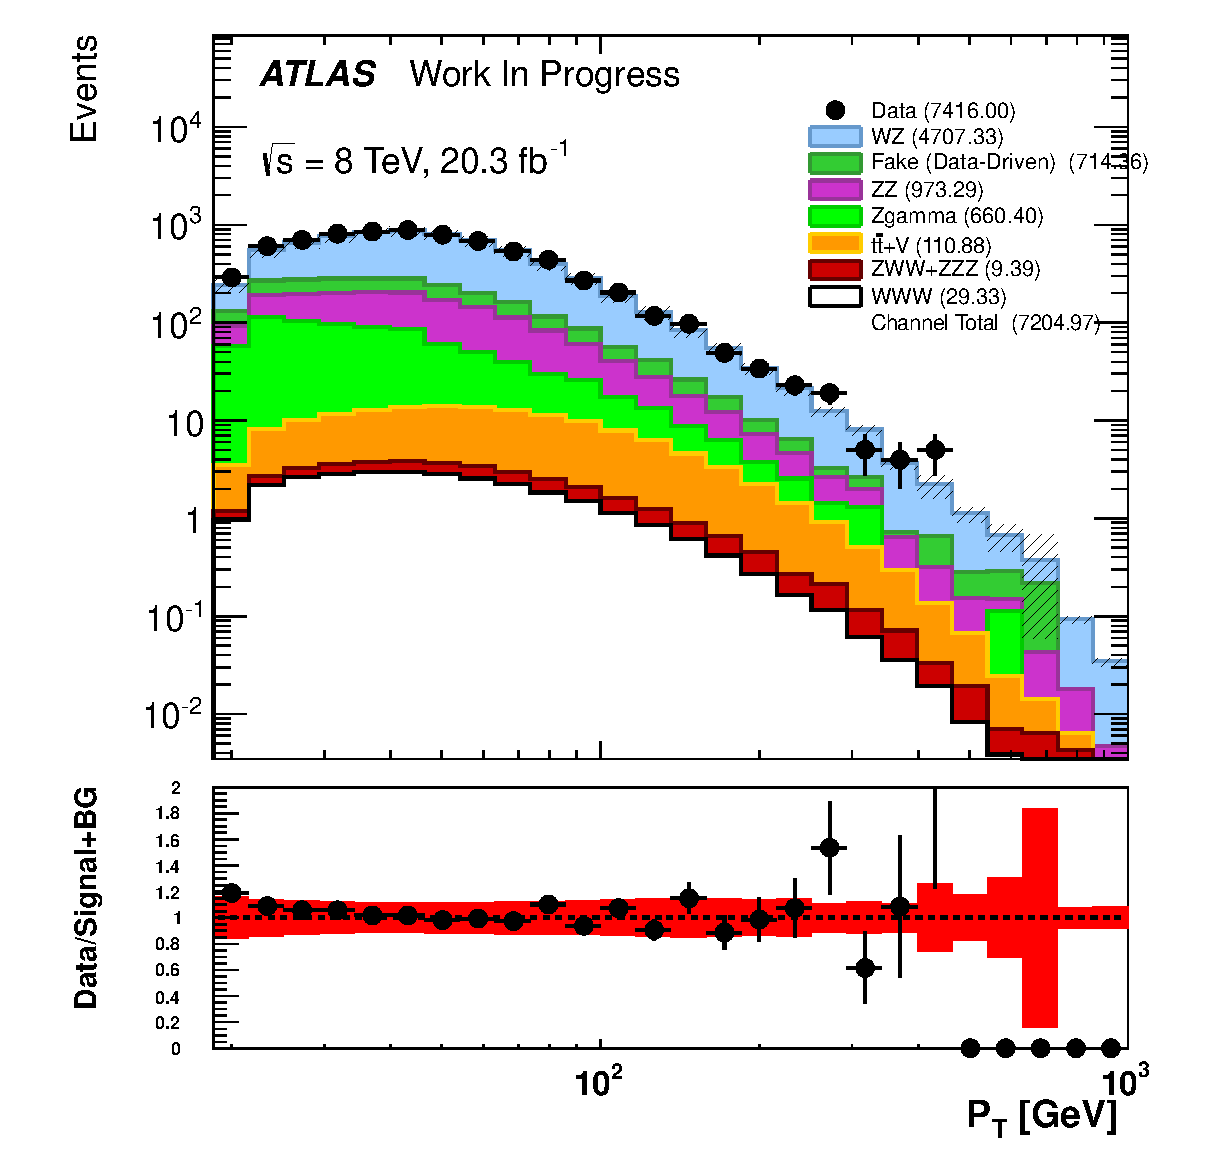
\includegraphics[width=0.3\columnwidth]{figures/appendix_signal_selection/Nov24Update_FakeSys_KFacSys_LogY_NoRebin/output/jobs/MxM/DataFull_Rates_May13_FakeRatesExactly2Loose_MuonMxMBJetGt0_ElBJetGt0SubtractPC_MxM/PreselectionNov23_15_physics/weight_all/eps/AllLeptonPt_histratio.eps}
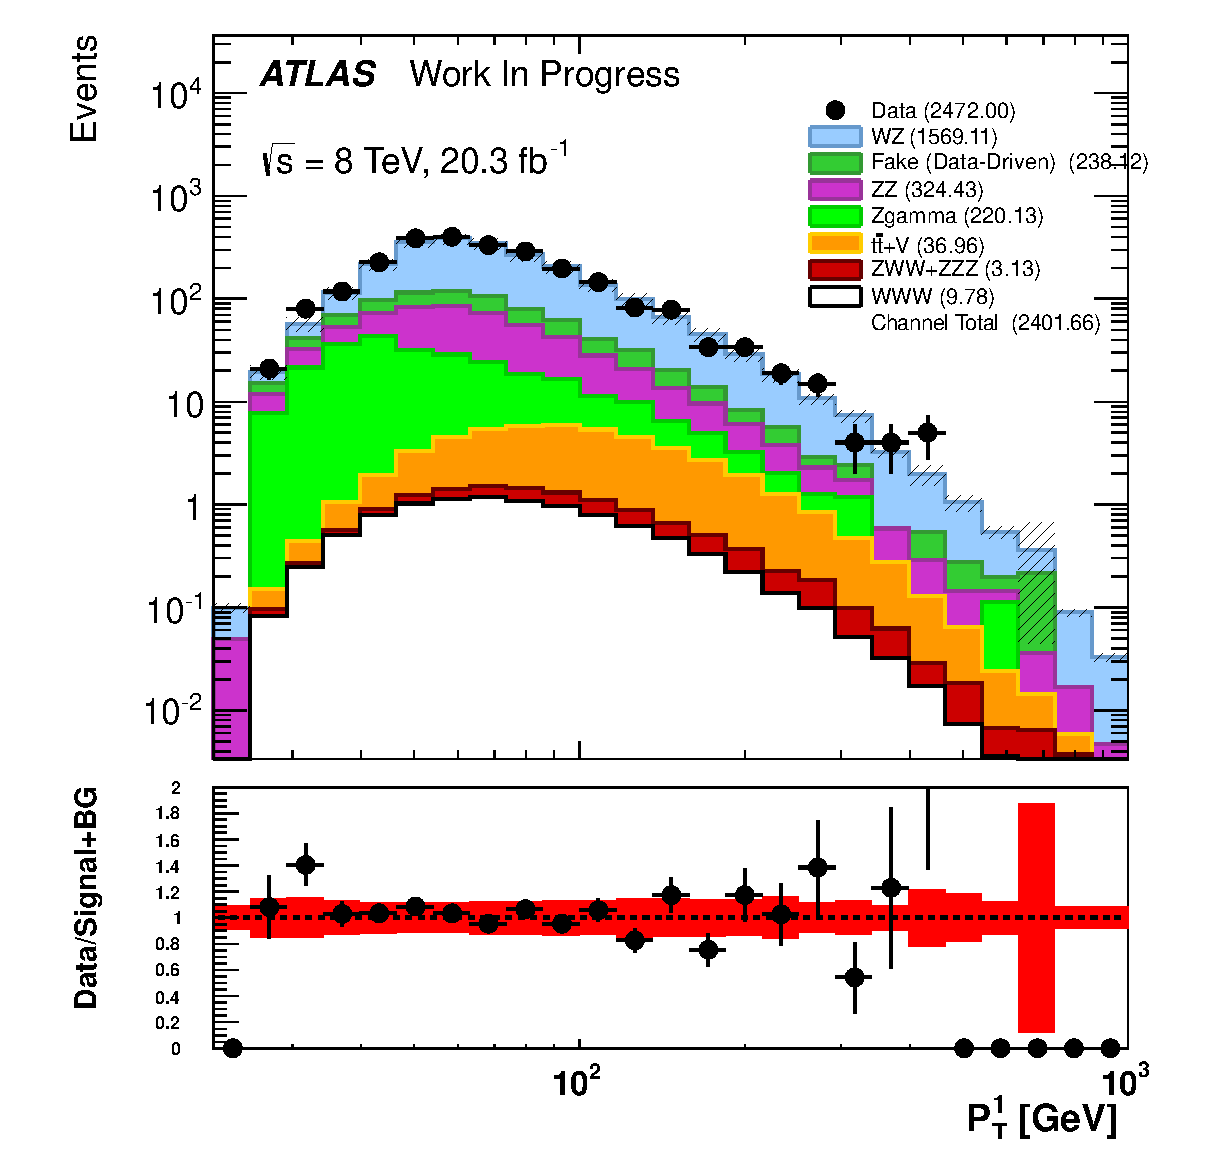
\includegraphics[width=0.3\columnwidth]{figures/appendix_signal_selection/Nov24Update_FakeSys_KFacSys_LogY_NoRebin/output/jobs/MxM/DataFull_Rates_May13_FakeRatesExactly2Loose_MuonMxMBJetGt0_ElBJetGt0SubtractPC_MxM/PreselectionNov23_15_physics/weight_all/eps/LeadingLeptonPt_histratio.eps}
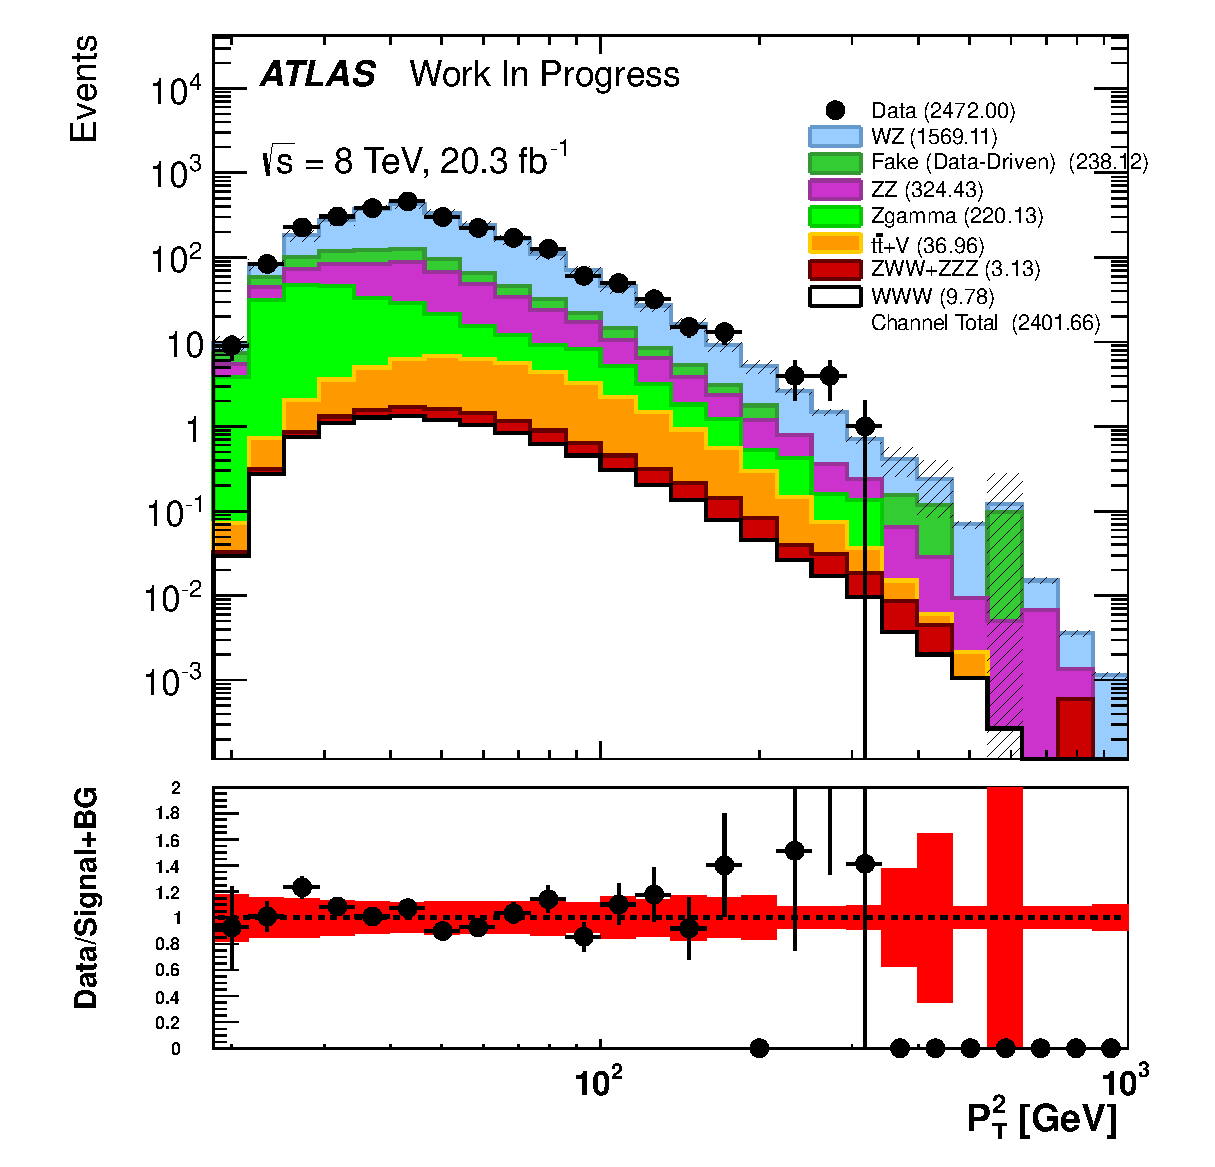
\includegraphics[width=0.3\columnwidth]{figures/appendix_signal_selection/Nov24Update_FakeSys_KFacSys_LogY_NoRebin/output/jobs/MxM/DataFull_Rates_May13_FakeRatesExactly2Loose_MuonMxMBJetGt0_ElBJetGt0SubtractPC_MxM/PreselectionNov23_15_physics/weight_all/eps/SubleadingLeptonPt_histratio.eps}
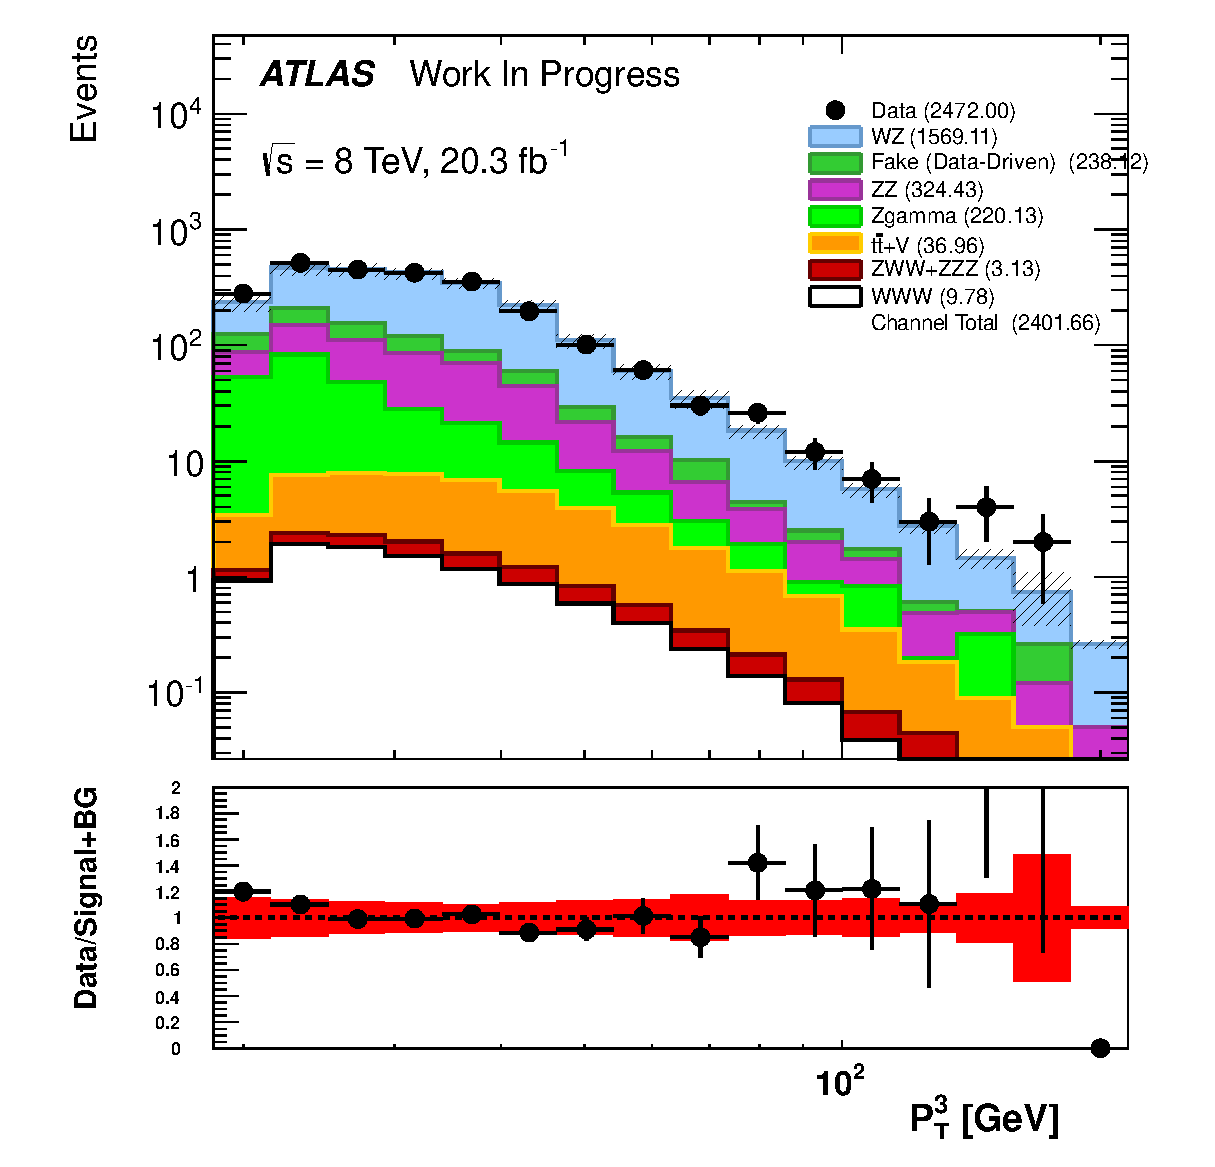
\includegraphics[width=0.3\columnwidth]{figures/appendix_signal_selection/Nov24Update_FakeSys_KFacSys_LogY_NoRebin/output/jobs/MxM/DataFull_Rates_May13_FakeRatesExactly2Loose_MuonMxMBJetGt0_ElBJetGt0SubtractPC_MxM/PreselectionNov23_15_physics/weight_all/eps/MinimumLeptonPt_histratio.eps}
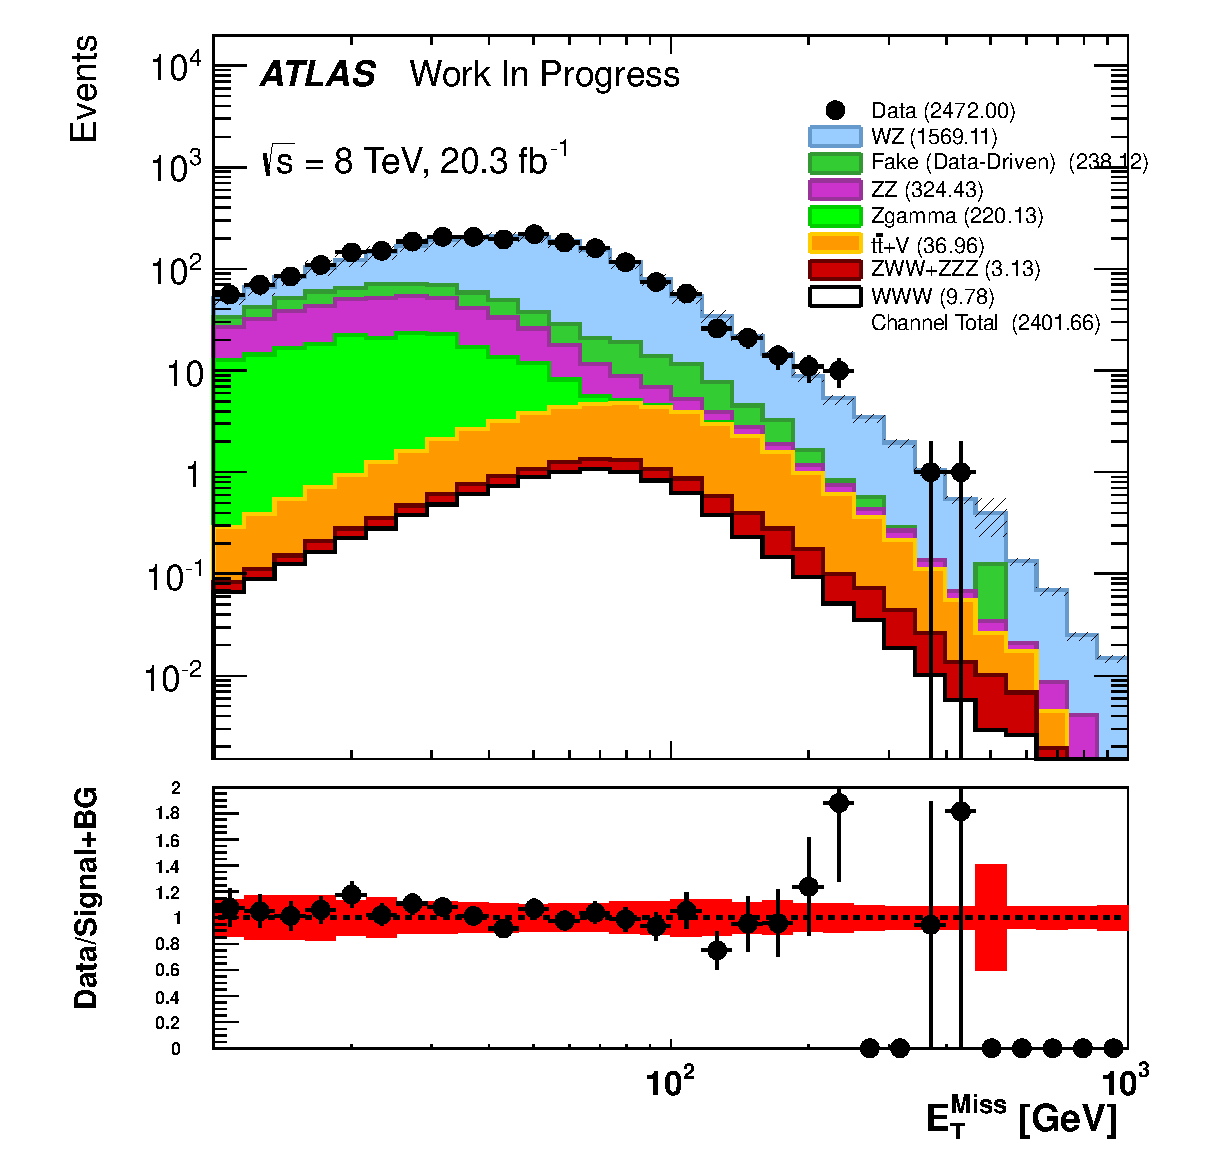
\includegraphics[width=0.3\columnwidth]{figures/appendix_signal_selection/Nov24Update_FakeSys_KFacSys_LogY_NoRebin/output/jobs/MxM/DataFull_Rates_May13_FakeRatesExactly2Loose_MuonMxMBJetGt0_ElBJetGt0SubtractPC_MxM/PreselectionNov23_15_physics/weight_all/eps/MET_Et_histratio.eps}
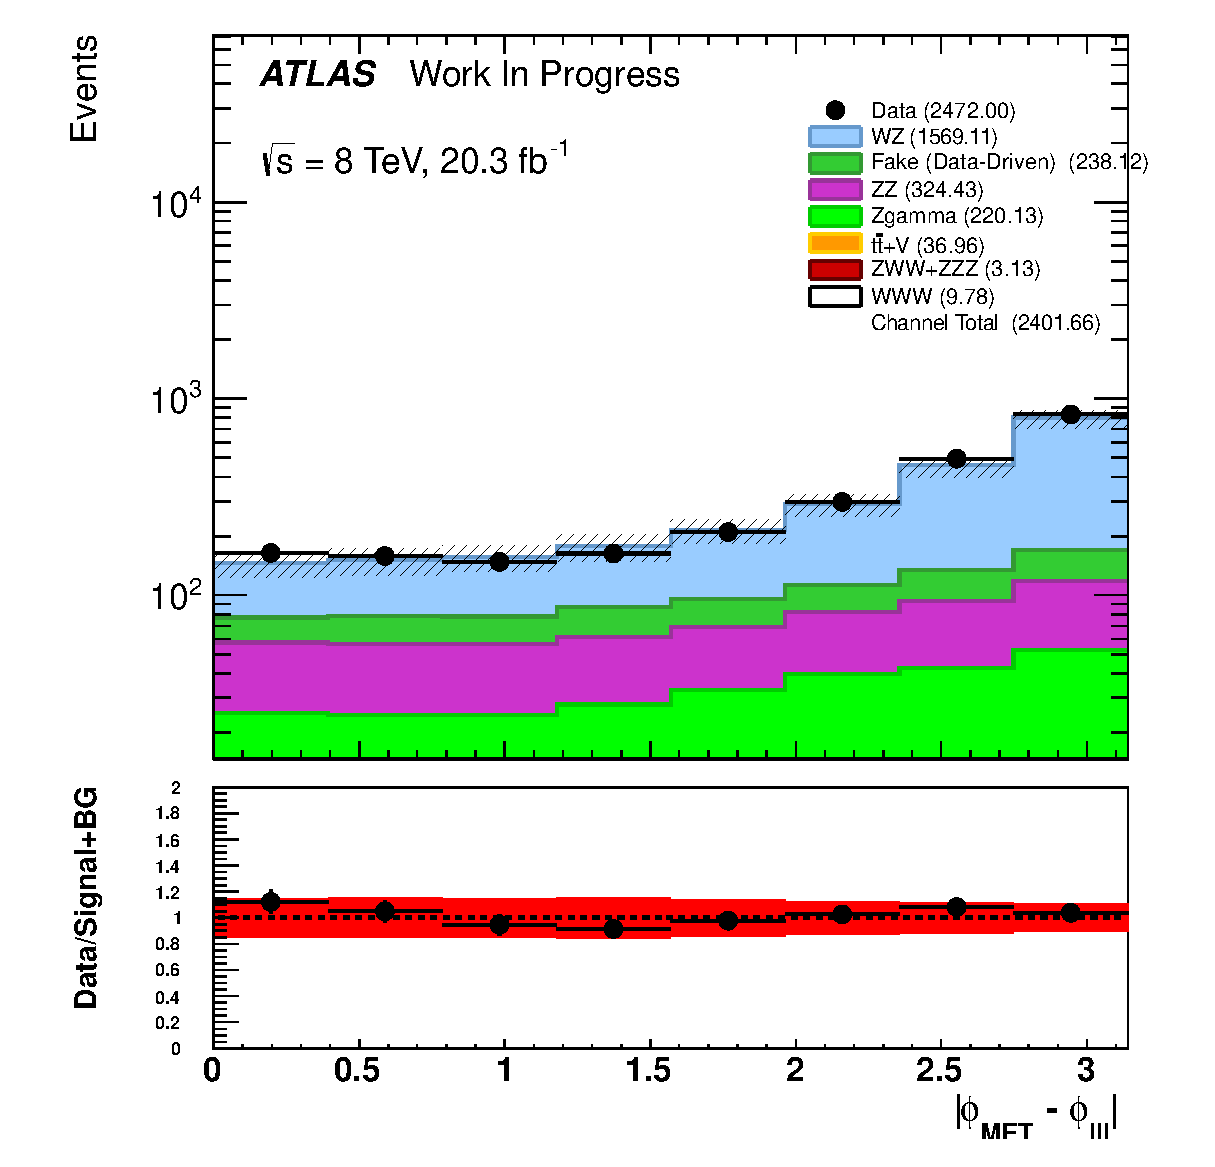
\includegraphics[width=0.3\columnwidth]{figures/appendix_signal_selection/Nov24Update_FakeSys_KFacSys_LogY_NoRebin/output/jobs/MxM/DataFull_Rates_May13_FakeRatesExactly2Loose_MuonMxMBJetGt0_ElBJetGt0SubtractPC_MxM/PreselectionNov23_15_physics/weight_all/eps/DeltaPhiMET123_Abs_histratio.eps}
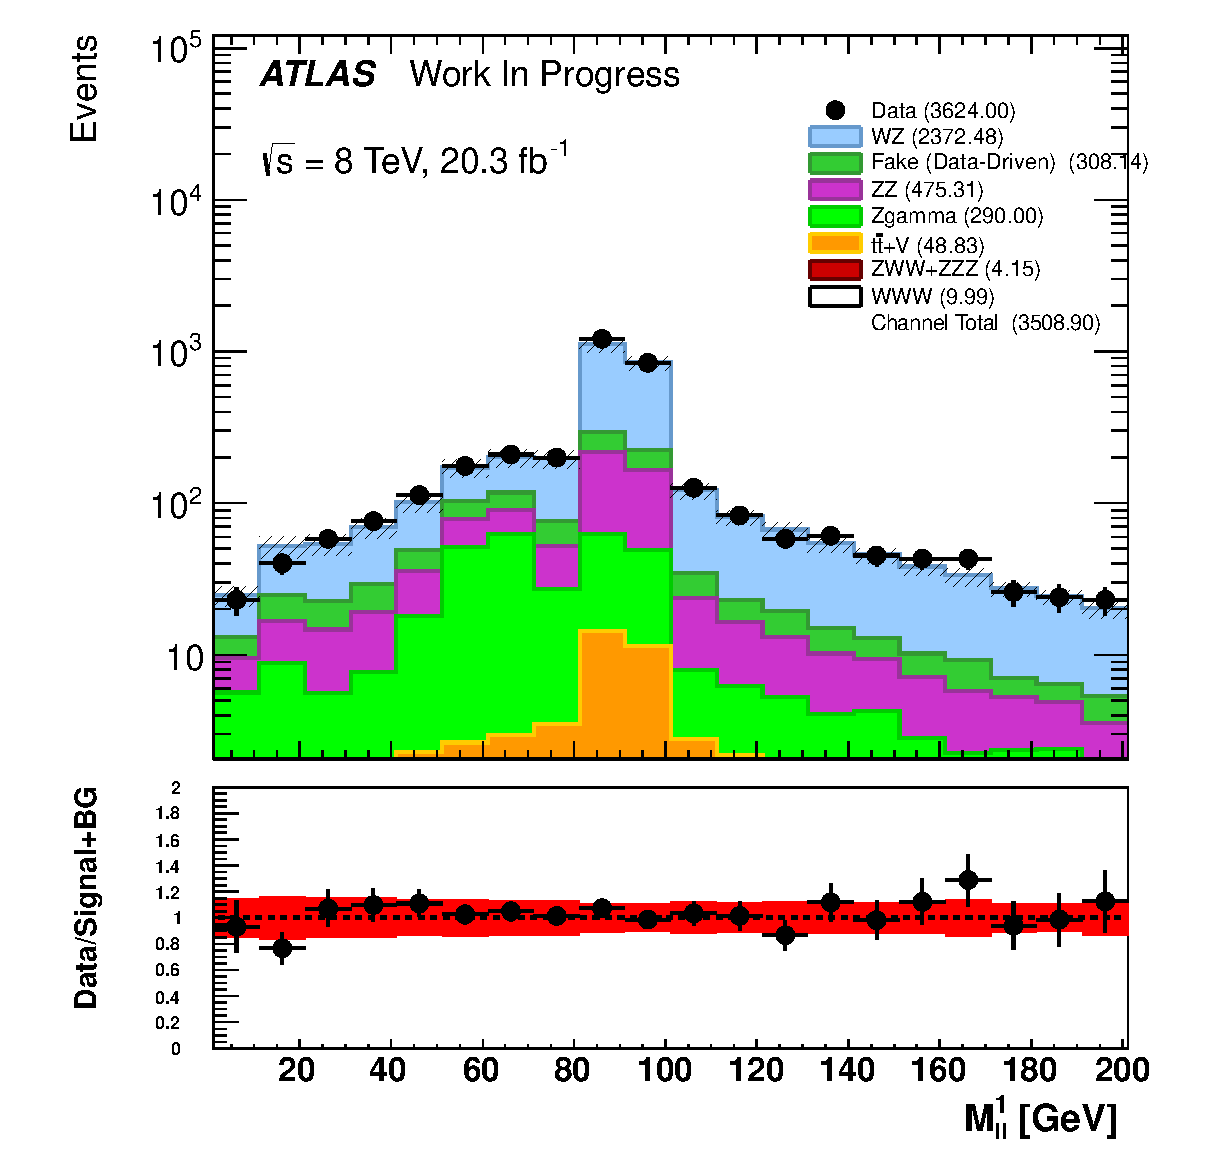
\includegraphics[width=0.3\columnwidth]{figures/appendix_signal_selection/Nov24Update_FakeSys_KFacSys_LogY_NoRebin/output/jobs/MxM/DataFull_Rates_May13_FakeRatesExactly2Loose_MuonMxMBJetGt0_ElBJetGt0SubtractPC_MxM/PreselectionNov23_15_physics/weight_all/eps/InvariantMassSFOS_histratio.eps}
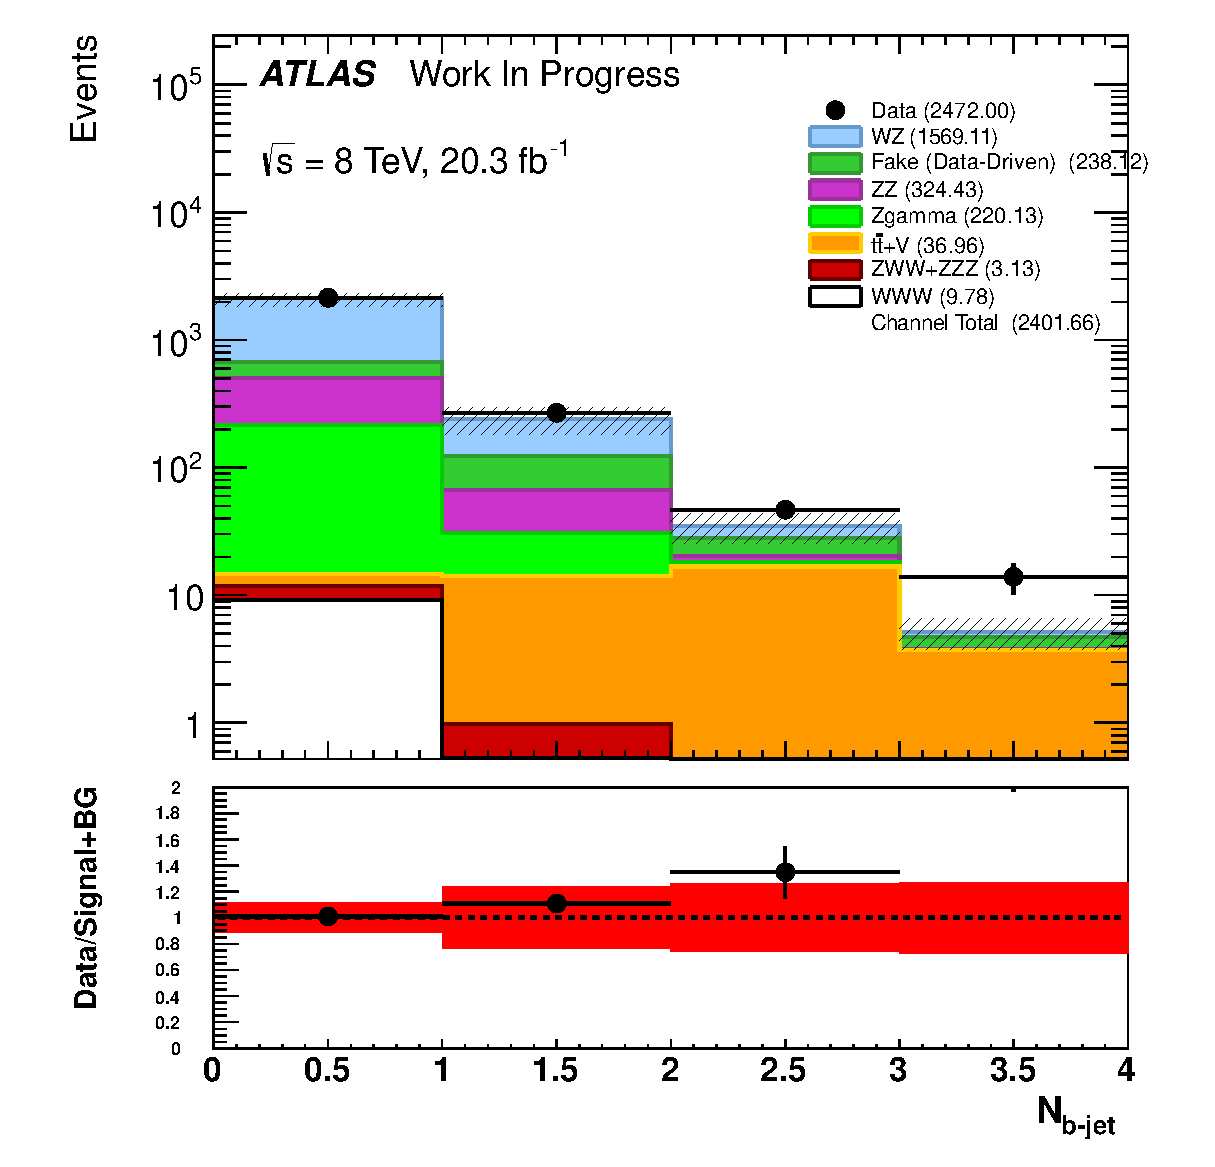
\includegraphics[width=0.3\columnwidth]{figures/appendix_signal_selection/Nov24Update_FakeSys_KFacSys_LogY_NoRebin/output/jobs/MxM/DataFull_Rates_May13_FakeRatesExactly2Loose_MuonMxMBJetGt0_ElBJetGt0SubtractPC_MxM/PreselectionNov23_15_physics/weight_all/eps/NBTaggedJets_histratio.eps}
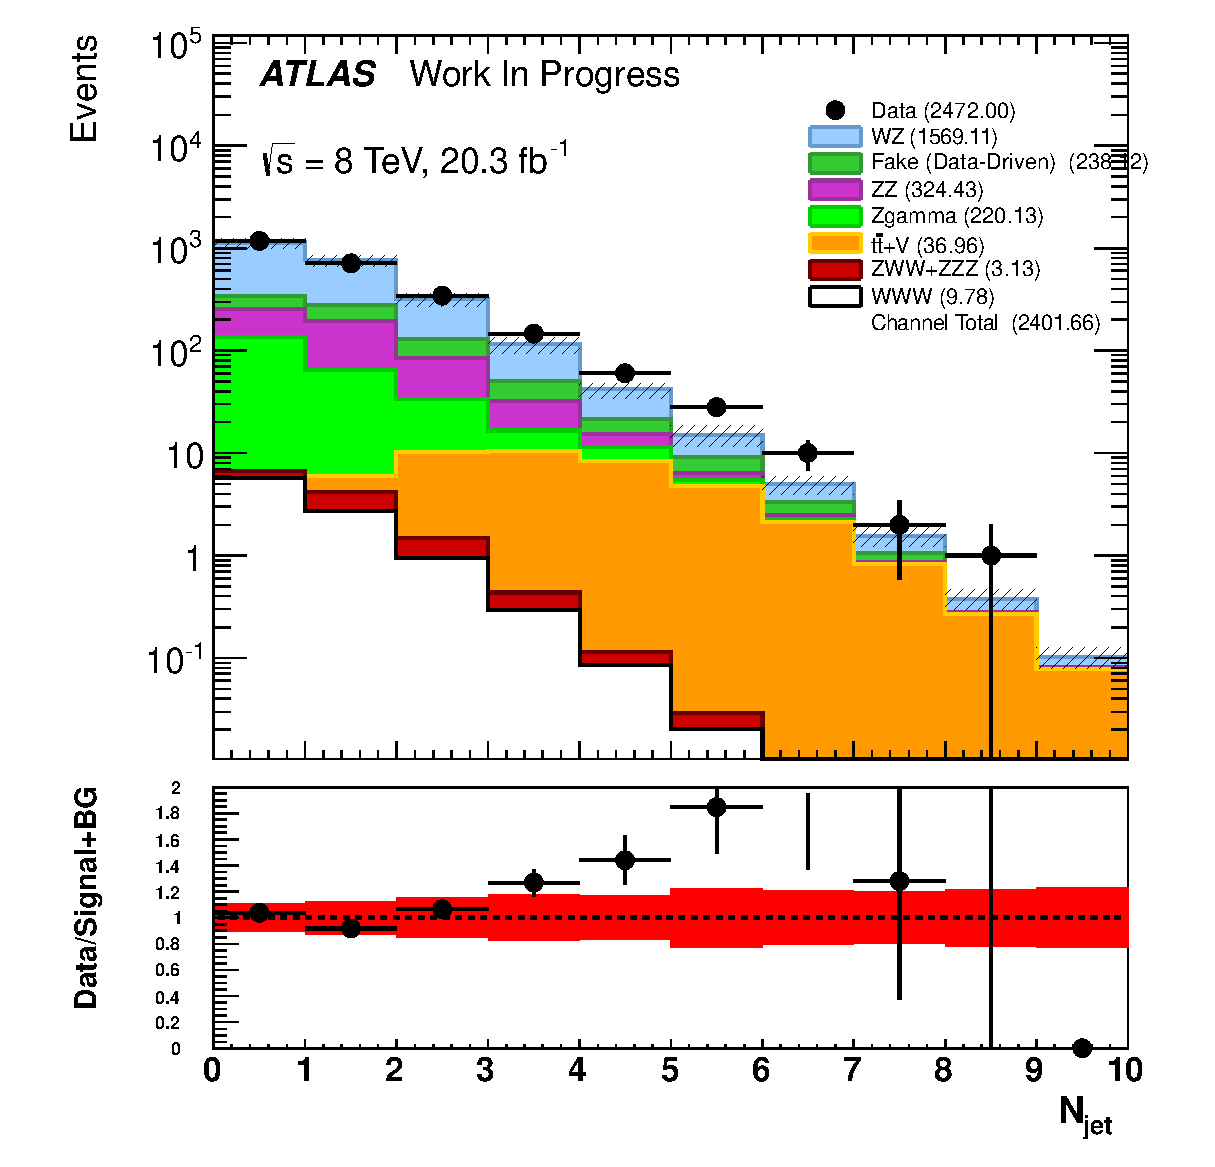
\includegraphics[width=0.3\columnwidth]{figures/appendix_signal_selection/Nov24Update_FakeSys_KFacSys_LogY_NoRebin/output/jobs/MxM/DataFull_Rates_May13_FakeRatesExactly2Loose_MuonMxMBJetGt0_ElBJetGt0SubtractPC_MxM/PreselectionNov23_15_physics/weight_all/eps/NJets_histratio.eps}
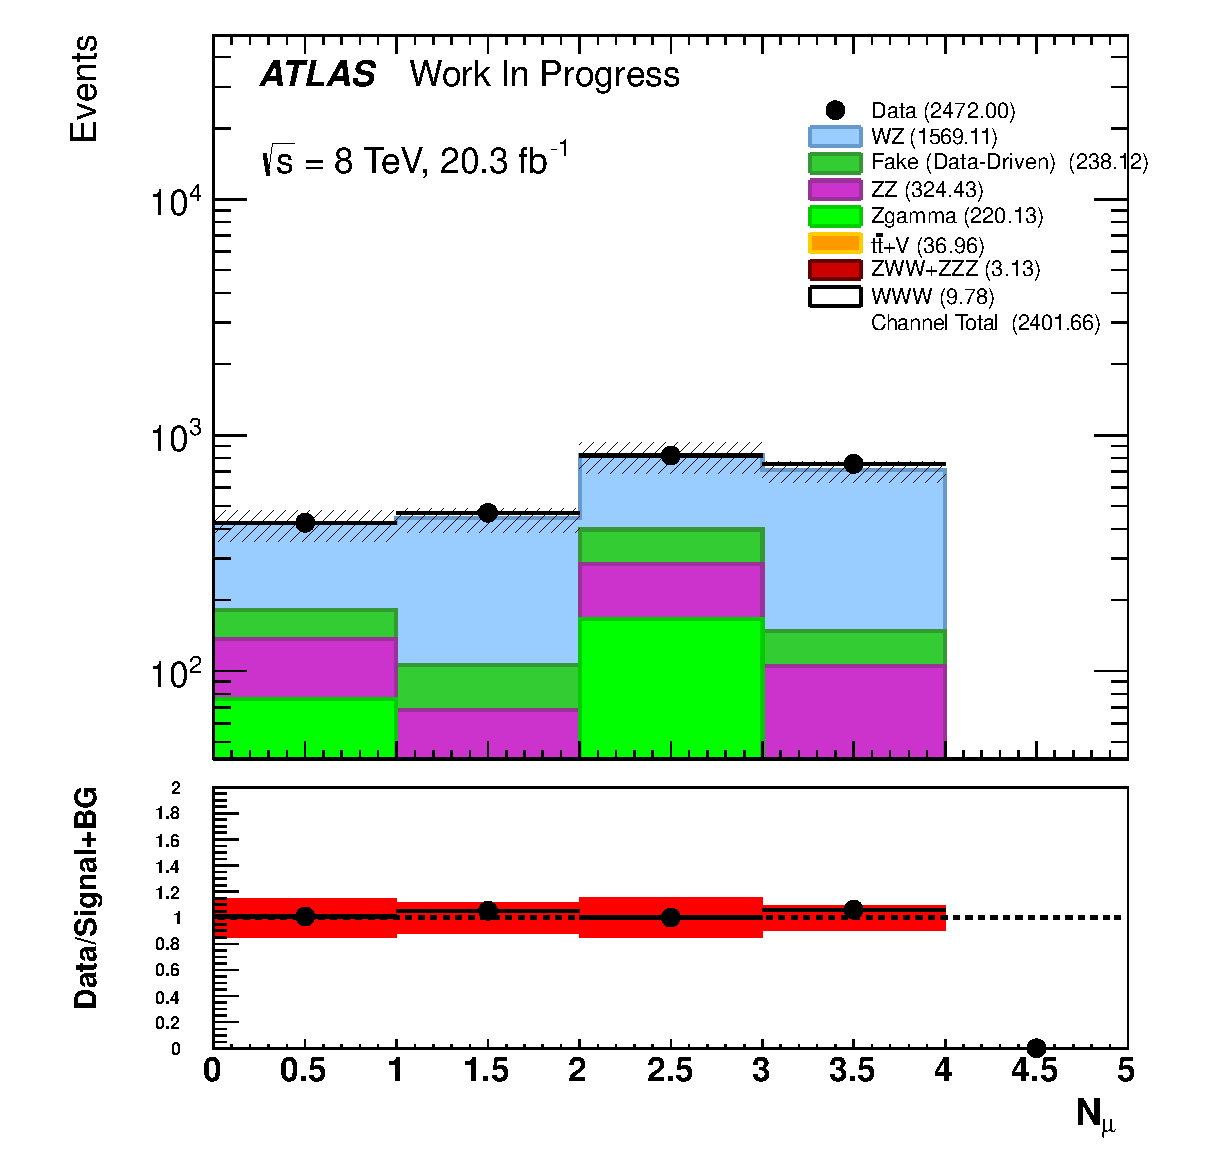
\includegraphics[width=0.3\columnwidth]{figures/appendix_signal_selection/Nov24Update_FakeSys_KFacSys_LogY_NoRebin/output/jobs/MxM/DataFull_Rates_May13_FakeRatesExactly2Loose_MuonMxMBJetGt0_ElBJetGt0SubtractPC_MxM/PreselectionNov23_15_physics/weight_all/eps/NMuons_histratio.eps}
%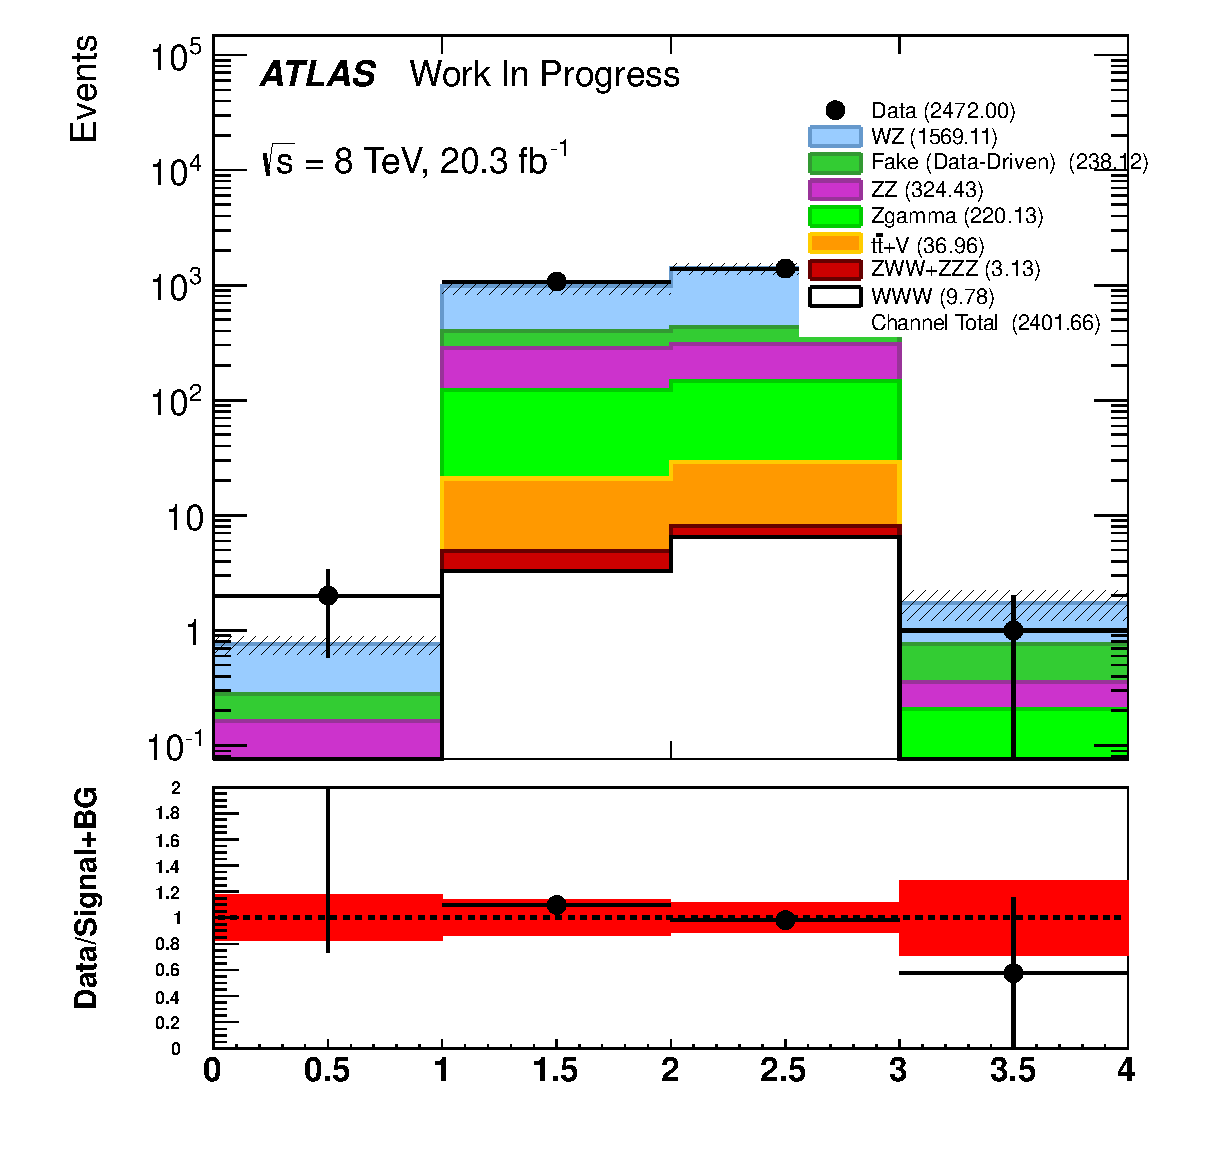
\includegraphics[width=0.3\columnwidth]{figures/appendix_signal_selection/Nov24Update_FakeSys_KFacSys_LogY_NoRebin/output/jobs/MxM/DataFull_Rates_May13_FakeRatesExactly2Loose_MuonMxMBJetGt0_ElBJetGt0SubtractPC_MxM/PreselectionNov23_15_physics/weight_all/eps/TotalCharge_histratio.eps}
\caption{Distributions showing the observed data compared to the background estimate at event pre-selection.}
\label{fig:preselection}
\end{figure}
The signal plus background model 
(described in detail in \sec\ref{sec:bg_estimates})
is compared to data at pre-selection
for a few different kinematic distributions of interest 
in \fig\ref{fig:preselection}. In the upper plot of each distribution,
the colored histograms 
represent the different categories contributing to the signal 
plus background model and 
are split by color based on the category. 
%The colors are...
Hashed bands are shown on the stacked
histograms representing the size of the systematic uncertainties 
on the model, described later in \sec\ref{}.
The data is shown in the black points where the 
bars on the points represent the statistical uncertainty on the data.
The lower plot shows the ratio of the data over the model.
In this case, the error bars correspond to the statistical uncertainty
on the ratio due to both the data and the model. The red band
shows the size of the systematic uncertainties with respect to the model.
The model is said to be consistent with the data
if the ratio is consistent with unity after considering statistical
and systematic uncertainties.
The different distributions are chosen primarily because 
of their potential to discriminate between signal and background. 
From top to bottom and left to right,
these distributions are: 
\begin{itemize}
\item Lepton $P_{T}^{1}$:  The momentum of the lepton in the transverse plane
which has the largest transverse momentum out of all three leptons selected.
\item Lepton $P_{T}^{2}$:  The momentum of the lepton in the transverse plane
which has the second largest transverse momentum out of all three leptons selected.
\item Lepton $P_{T}^{3}$:  The momentum of the lepton in the transverse plane
which has the smallest transverse momentum out of all three leptons selected.
\item \MET:  The missing transverse energy
\item $\Delta\varphi(lll,\MET)$:  The difference in the polar angle 
between the three lepton $p_{T}$, 
$\overrightarrow{p_{T}^{lll}} =  \overrightarrow{p_{T}^{1}}+ 
\overrightarrow{p_{T}^{2}}+ \overrightarrow{p_{T}^{2}}$, 
and \MET. It can be expressed as 
$\Delta\varphi(lll,\MET) = \cos^{-1}\frac{ \overrightarrow{p_{T}^{lll}}\cdot\overrightarrow{\MET} }{ p_{T}^{lll}\MET } $
\item SFOS Invariant Mass ($m_{\textrm{SFOS}}$): The di-lepton invariant mass
of each SFOS lepton pair in the event. %do i need to define the invariant mass?
\item Three Lepton $m_{T}$: The transverse mass of the three lepton system
and the missing transverse energy, or
$m_{T}^{lll} = \sqrt{2p_{T}^{lll}\MET(1-\cos(\Delta\varphi(lll,\MET)))}$ 
\item $N_{\textrm{Jet}}$: The number of jets selected in the event.
\item $N_{b-\textrm{Jet}}$: The number of \bee-jets tagged in the event.
\item $N_{\mu}$: The number of selected leptons that are muons. The maximum
possible is 3. If the lepton is not a muon it must be an electron.
\end{itemize}
In general, the signal plus background model is observed to be consistent
with the data at the pre-selection, at least for those distributions
considered here.



\subsection{Signal Region Selection}
\label{sec:signal_regions}
The signal regions used in this analysis are separated based on the number of 
Same-Flavor Opposite-Sign (SFOS) lepton pairs selected in the event.  That is to say,
the number of lepton pair combinations in the event 
which could feasibly come from the leptonic decay of a $Z$-boson.
This results in three separate signal regions listed 
below with the lepton charge combinations
that fall in each category:
\begin{itemize}
\item \textbf{0 SFOS}: $e^{\pm}e^{\pm}\mu^{\mp}$, 
$\mu^{\pm}\mu^{\pm}e^{\mp}$ ($e^{\pm}e^{\pm}\mu^{\pm}$, 
$\mu^{\pm}\mu^{\pm}e^{\pm}$, $e^{\pm}e^{\pm}e^{\pm}$, $\mu^{\pm}\mu^{\pm}\mu^{\pm}$)
\item \textbf{1 SFOS}: $e^{\pm}e^{\mp}\mu^{\pm}$, 
$e^{\pm}e^{\mp}\mu^{\mp}$, $\mu^{\pm}\mu^{\mp}e^{\pm}$, $\mu^{\pm}\mu^{\mp}e^{\mp}$
\item \textbf{2 SFOS}: $e^{\pm}e^{\pm}e^{\mp}$, $\mu^{\pm}\mu^{\pm}\mu^{\mp}$
\end{itemize}
Note that in the 2 SFOS region, one lepton is allowed to belong to both 
pair combinations.
Those combinations listed in parentheses are not allowed for the signal based on charge conservation (neglecting charge mis-identification).  
The amount of the $W^{\pm}W^{\mp}W^{\pm}$ signal
which falls into each category is purely combinatoric.  
From the above list one can thus see that there are twice as many ways 
for the signal combinations (again neglecting those in parentheses)
to fall in the 1 SFOS regions as 
there to fall in either the 0 SFOS or 2 SFOS regions. 
Absent possible differences in signal efficiencies based on the leptons in each 
signal region, one should expect branching 
fractions of 25\%, 50\% and 25\% for the 0, 1, and 2 SFOS signal regions, respectively.


\begin{figure}[ht!]
\centering
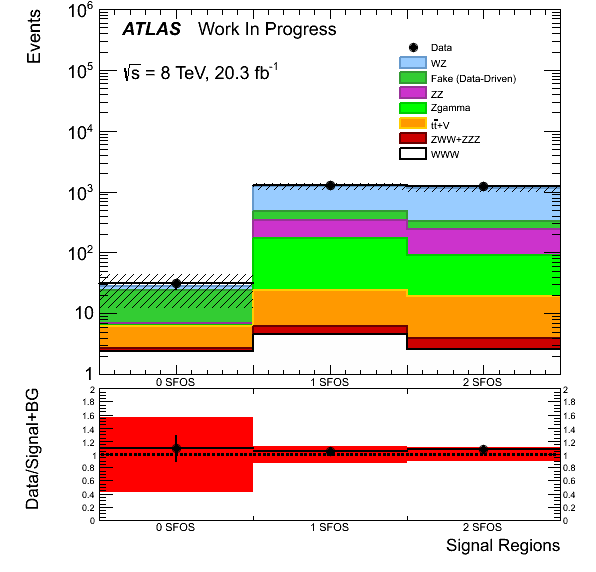
\includegraphics[width=0.5\columnwidth]{figures/SFOSPreselection.png}
\caption{Yields at event pre-selection in the 0, 1 and 2 SFOS regions.  
The most important systematic uncertainties 
(discussed in section~\ref{sec:systematics}) are shown, 
namely from the fake estimates and the uncertainties on the WZ and ZZ k-factors.}
\label{fig:preselection_nsfos}
\end{figure}

Indeed, upon splitting the pre-selection region based on the number of SFOS
pairs, we end up with signal and background predictions like in 
\fig\ref{fig:preselection_nsfos}, where we can see difference
in branching fraction for the signal to each of the three signal regions.
In the 0 and 2 SFOS regions, roughly 2.5 signal events are predicted
whereas closer to 5 signal events are predicted in the 1 SFOS region. 
Totaling about 10 signal events predicted at the pre-selection stage.
Shifting to looking at the background, perhaps the most striking 
feature of this plot is the 
clear difference in background yield and background composition
between the 0 SFOS region and the 1 and 2 SFOS regions.
More than 1000 background events are predicted in both the 1 and
the 2 SFOS regions, while only about 30 background events are
predicted in the 0 SFOS region.
Apparently then, the advantage of splitting the signal region based on this
classification comes when looking at the background, specifically the
electroweak $WZ$ and $ZZ$ backgrounds where SFOS lepton pairs may be
produced from the decay of the $Z$ boson(s). Consider only the case
where the $WZ$ and $ZZ$ decay to either $e$ or $\mu$.  The $WZ$ production
process is thus characterized by 3 leptons with at least 1 SFOS lepton pair
which comes from the $Z$. If all three leptons from the $WZ$ decay have been
reconstructed, then there is a 50~\% chance the third lepton 
will also be able to form a SFOS pair with one of the leptons from the $Z$ decay.
Thus, the WZ background will split evenly between the 1 and 2 SFOS classification.
Something similar occurs for the ZZ background except that the fourth lepton 
in the decay must be lost (usually due to possessing a low $\pt$).
The large cross-section for theses processes means that
they become the dominant backgrounds in the 1 and 2 SFOS regions.  
The 0 SFOS signal region is mostly spared from contamination  by 
these large processes but still
includes both the $WZ$ and $ZZ$ processes as background due to the
non-negligible (albeit small) effect of mis-measurement of the lepton
charge, see section~\ref{sec:chargeMisID}.  The 0 SFOS signal region
is thus unique in having a small background which is almost entirely
reducible and dominated instead by events where a jet is mis-measured
as or overlaps with a lepton, called the fake lepton background, along
with the aforementioned sub-dominant effect of lepton charge 
mis-identification described in Section~\ref{sec:chargeMisID}.  
From this, one can clearly see that it is
advantageous to split these signal regions so that the dominant
backgrounds in each region may be targeted individually.  Furthermore,
note that while the 1 SFOS region contains more of the signal than the
0 and 2 SFOS regions, it is the 0 SFOS region which is most likely to
have the best sensitivity due to the smaller background contribution.


Within each signal region it may be that we can further reduce the 
background with respect to the signal region. 
By restricting to a region of phase space which removes a larger
fraction of background than it does the signal, we can 
increase the signal prediction with respect to the background.
The ratio of events which pass a selection with respect
to the original number of events is referred to as the 
efficiency.
Thus, we refer to this as choosing a selection threshold where 
the signal efficiency is larger than the background efficiency.
Because the background composition in the 0 SFOS region
is so different from the 1 and 2 SFOS regions, it is likely that
the selection which does this will also differ between them. 
And even though the
1 and 2 SFOS regions are reasonably similar, we should not rule out
the possibility that they also have a uniquely optimal selection.
Based on heuristic arguments, a list of reasonable physical
quantities to restrict were considered. The most promising of these quantities
are those listed previously in \sec\ref{sec:preselection}. 
Also, because the predicted amount of signal is so precious,
the signal efficiency should be kept as close to unity as possible.
Consider the following selection choices using the quantities defined
earlier:
%Do I need to add more plots here???
\begin{itemize}
\item Lepton $P_{T}$:  Require that exactly three leptons passing tight object quality requirements have a $P_{T} > X$.
\item Missing $E_{T}$:  Require that $\MET > X$.
\item $\Delta\varphi(lll,\MET)$:  Require that $\Delta\varphi(lll,\MET) = \cos^{-1}\frac{ \overrightarrow{p_{T}^{lll}}\cdot\overrightarrow{\MET} }{ p_{T}^{lll}\MET } > X$.
\item Jet Veto: Require that $N_{Jet} \leq X$.
\item b-Jet Veto: Require that $N_{b-Jet} \leq X$.
%\item Z Veto: Require that $m_{ll}$ does not fall in the region $m_{Z}-m_{min} < m_{ll} < m_{Z}-m_{max}$ where $m_Z = 91.1876$~GeV and where $m_{min}$ are $m_{max}$ are the boundaries of the \z-window with which to veto.  For the 1 and 2 SFOS regions the pairs used to construct the $m_{ll}$ are SFOS pairs of either electrons or muons.  In the 0 SFOS region there are no SFOS pairs by definition but there is still a \z-peak in the same-sign di-electron mass spectrum due to charge mis-id. Thus, in the 0 SFOS region we consider instead
\item Three Lepton $m_{T}$: Require that $m_{T}^{lll} > X$
%\item Same-flavor mass: Consider cuts on $m_{SF} > m_{min}$ and/or $m_{SF} < m_{max}$ where $m_{SF}$ is the invariant mass of same-flavor pairs (with no requirement on the sign) %what about this one?
\end{itemize}

\begin{figure}[ht!]
\centering
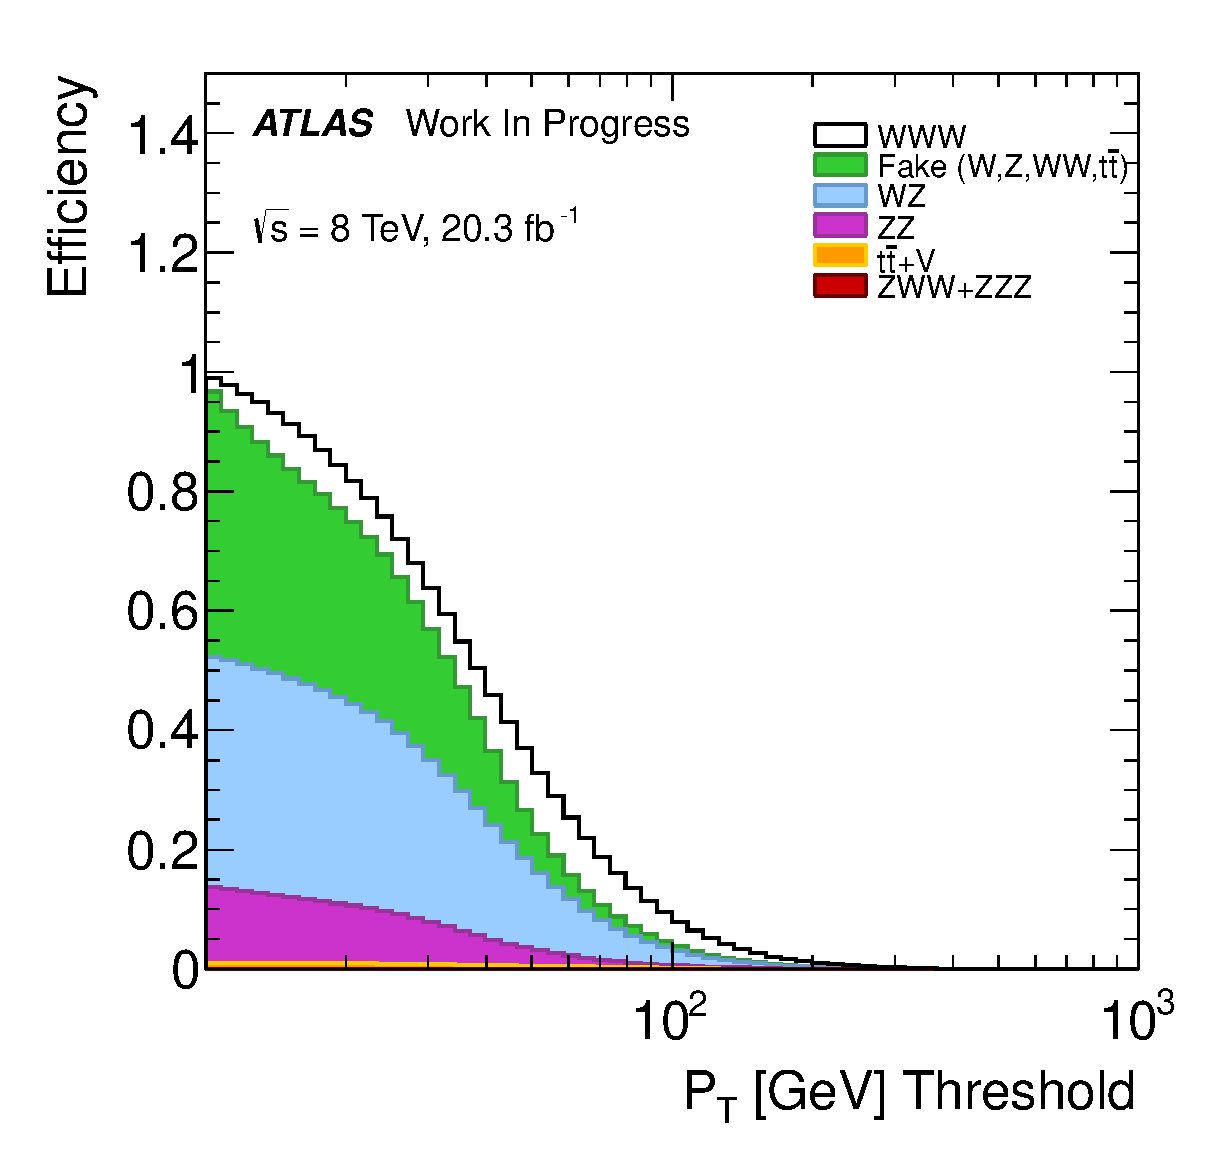
\includegraphics[width=0.3\columnwidth]{figures/optimization/SignalRegions_0p5mmZ0_Preselection_Efficiencies/AllLeptonPt_Cumulative.eps}
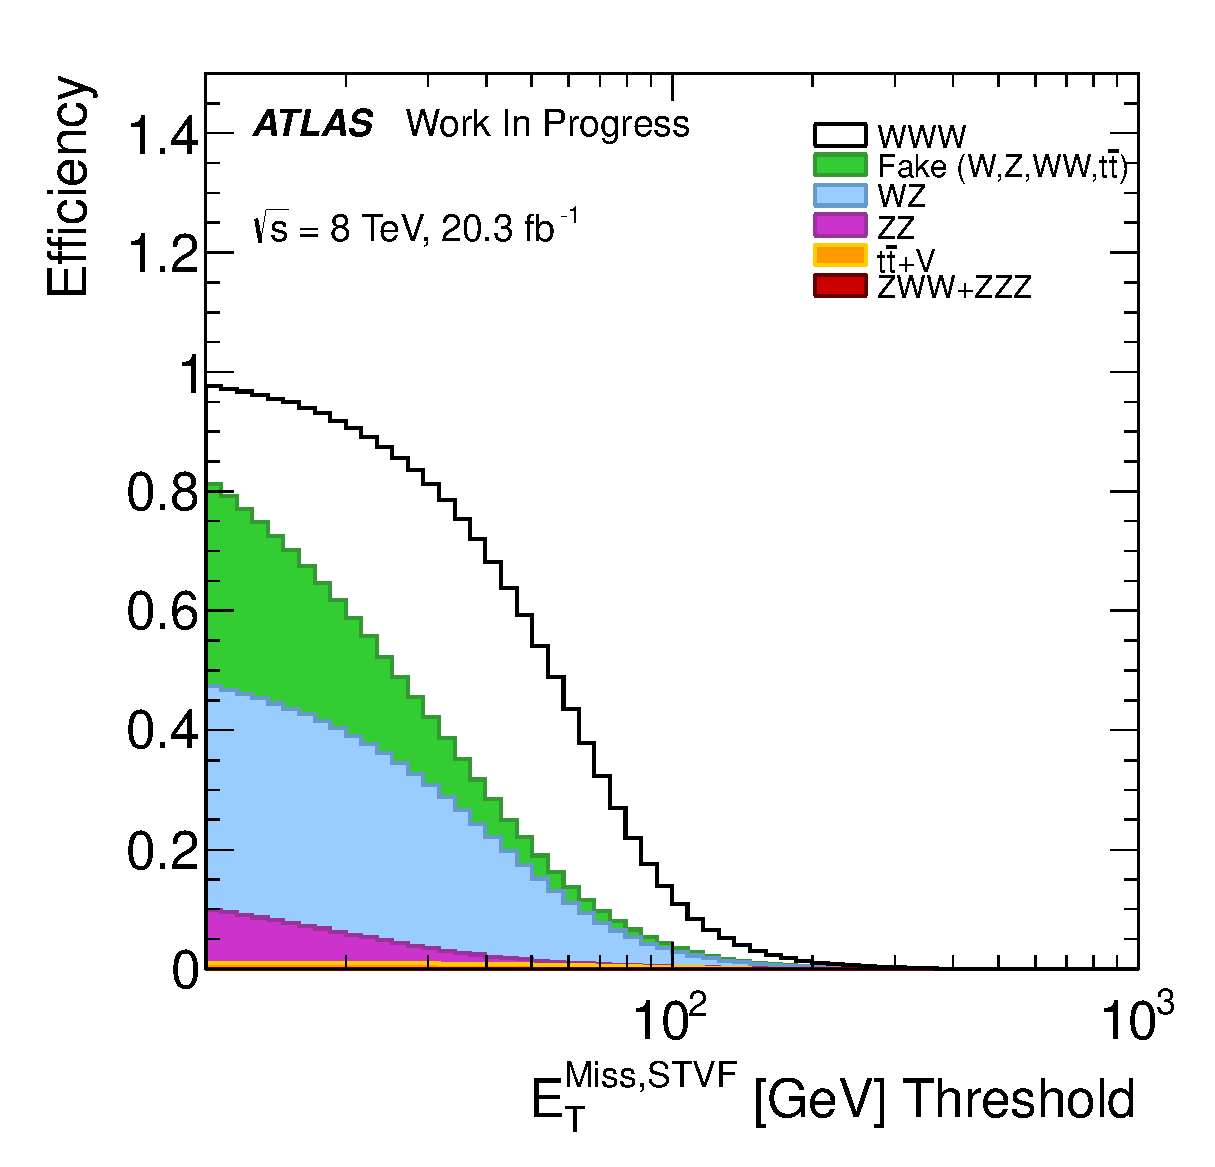
\includegraphics[width=0.3\columnwidth]{figures/optimization/SignalRegions_0p5mmZ0_Preselection_Efficiencies/MET_Et_STVF_Cumulative.eps}
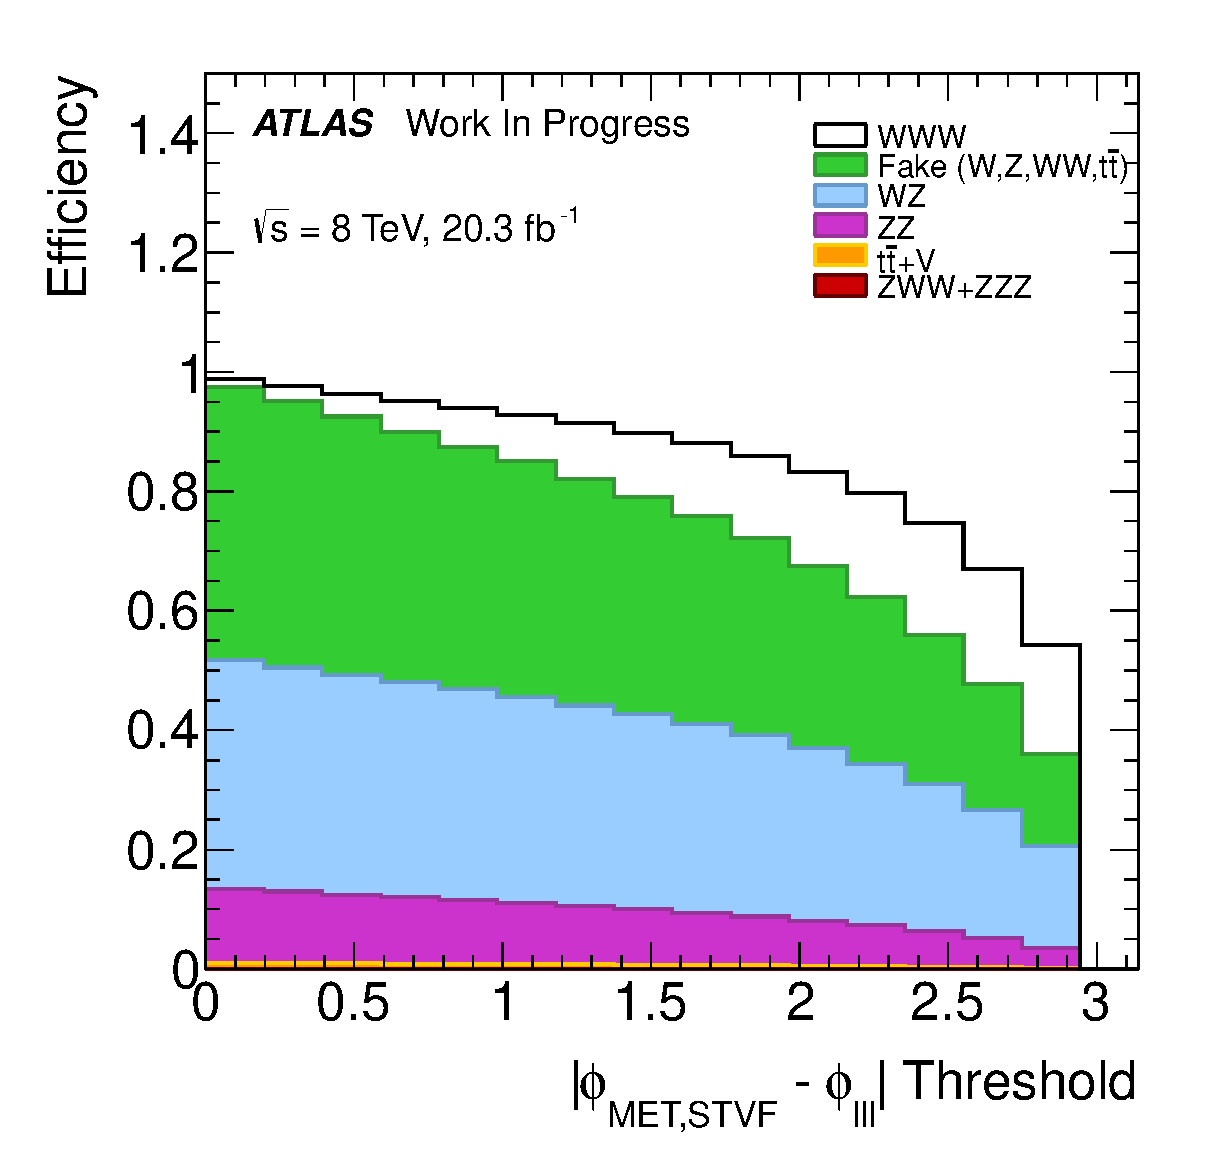
\includegraphics[width=0.3\columnwidth]{figures/optimization/SignalRegions_0p5mmZ0_Preselection_Efficiencies/DeltaPhiMETSTVF123_Abs_Cumulative.eps}
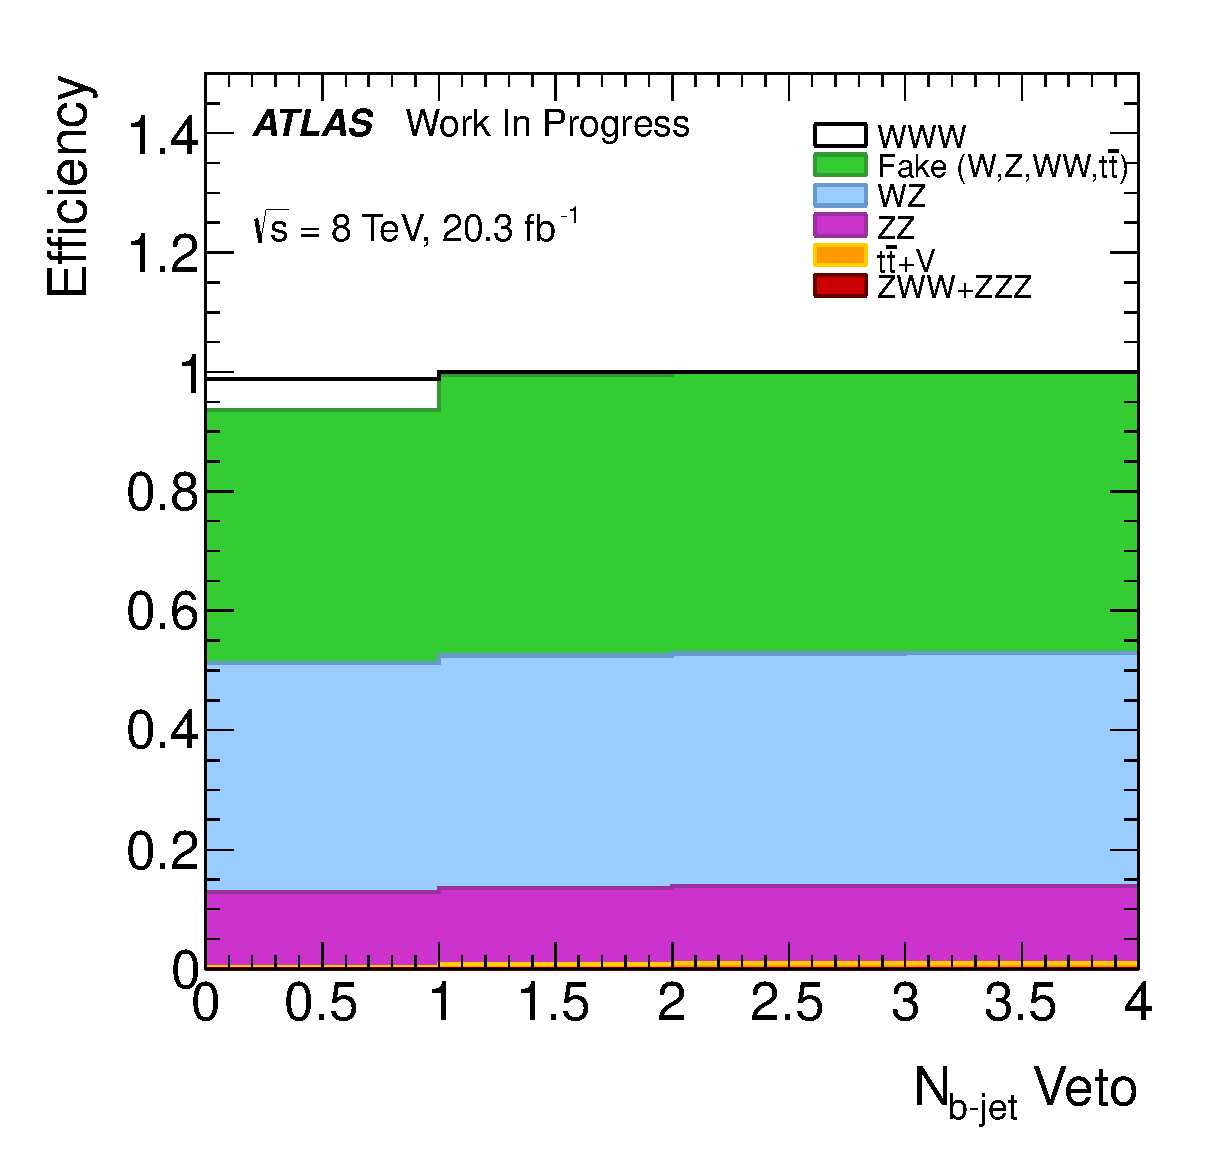
\includegraphics[width=0.3\columnwidth]{figures/optimization/SignalRegions_0p5mmZ0_Preselection_Efficiencies/NBTaggedJets_LeftCumulative.eps}
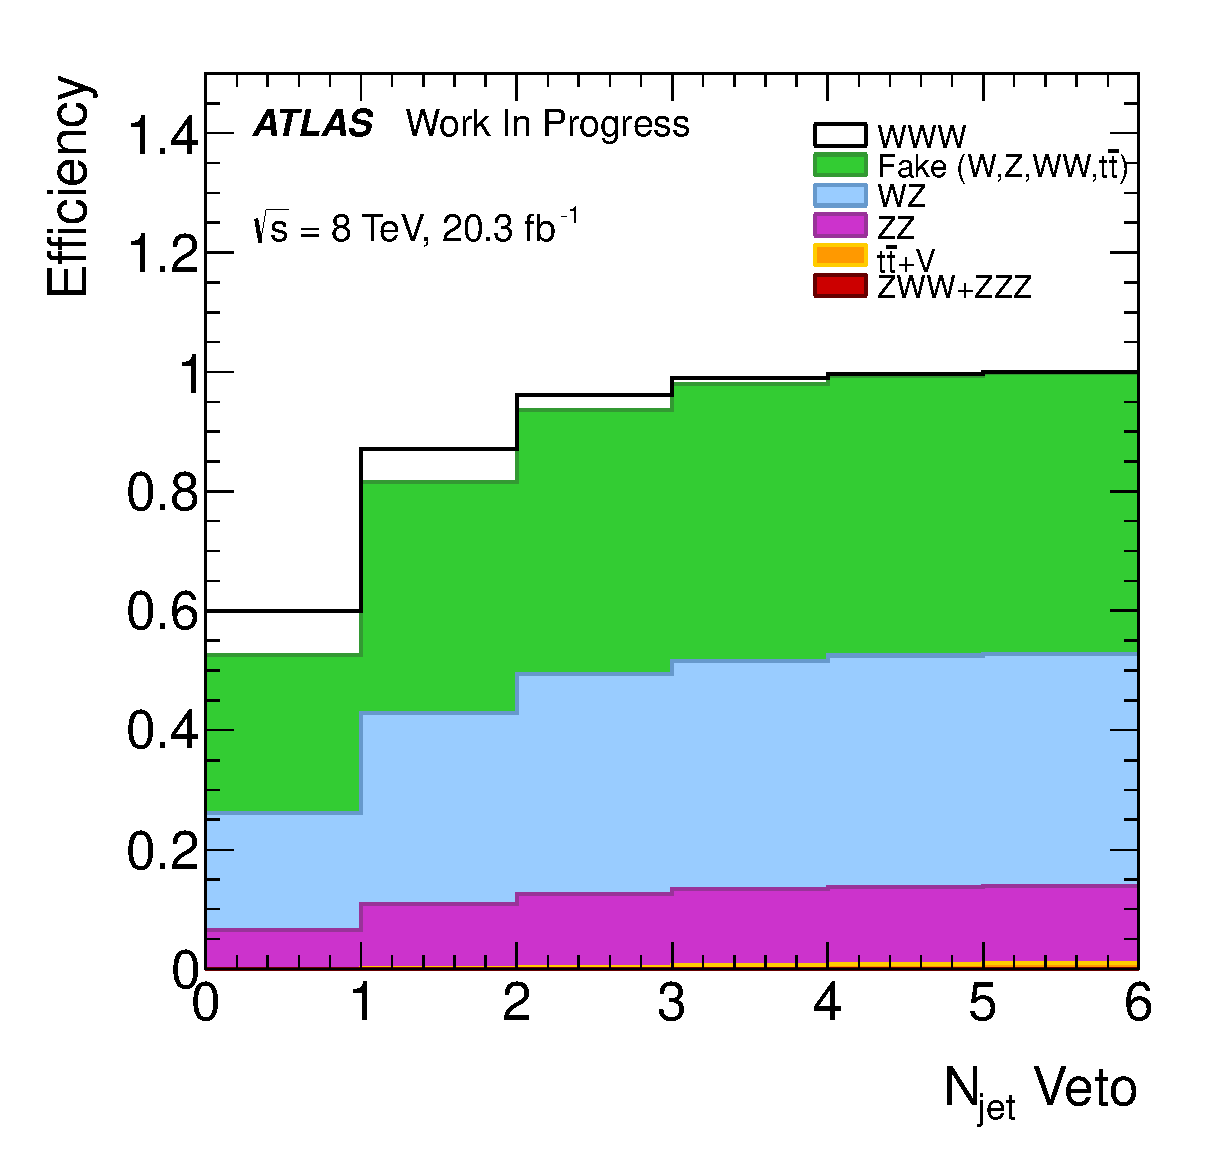
\includegraphics[width=0.3\columnwidth]{figures/optimization/SignalRegions_0p5mmZ0_Preselection_Efficiencies/NJets_LeftCumulative.eps}
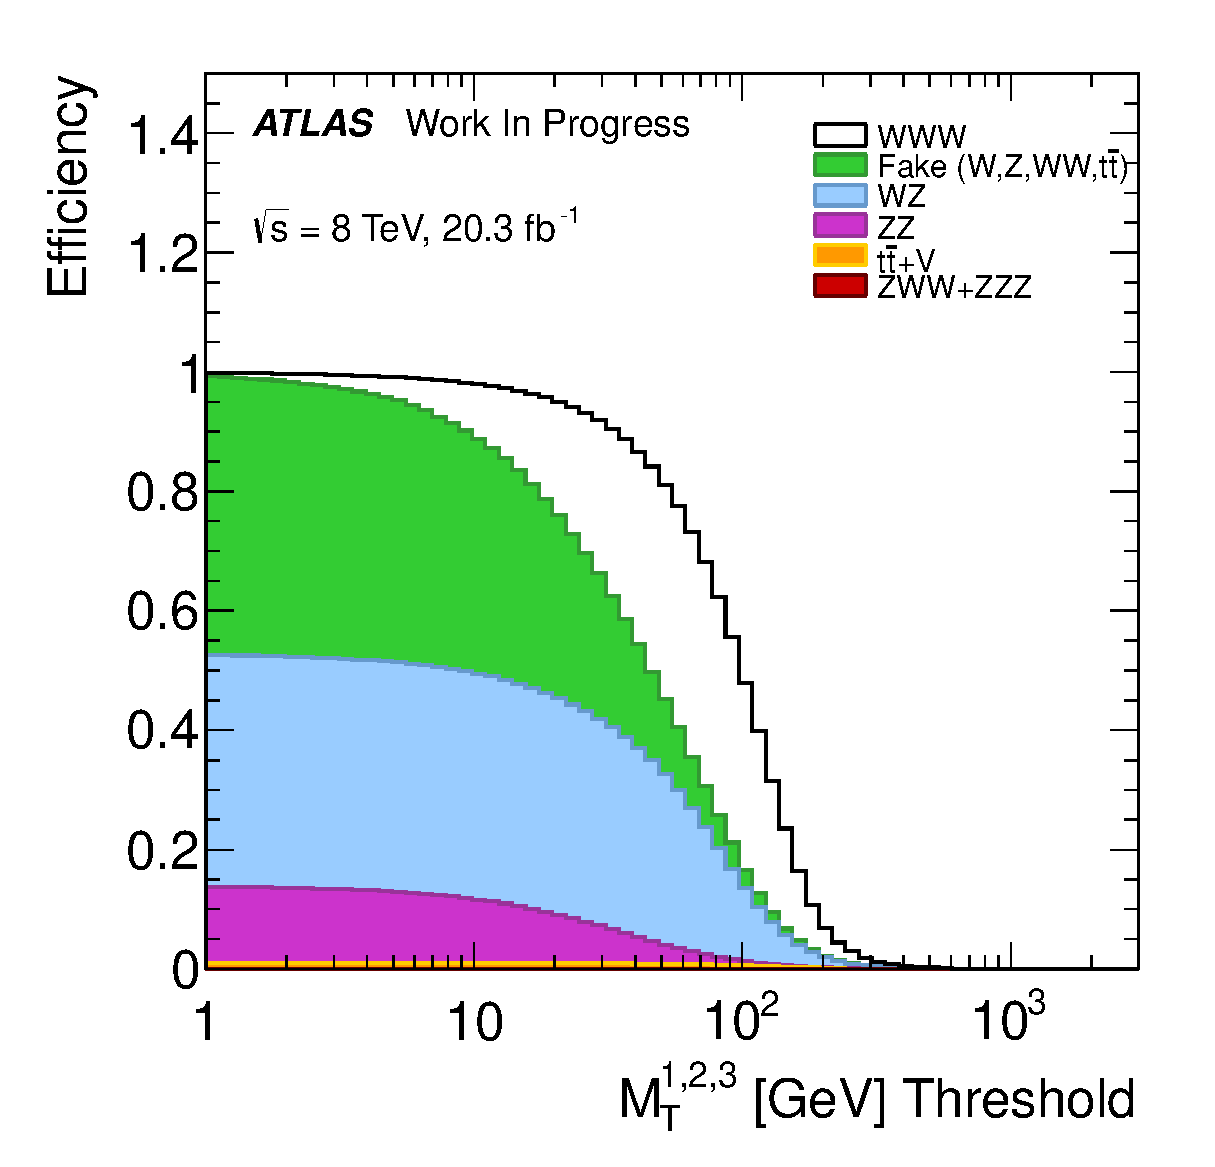
\includegraphics[width=0.3\columnwidth]{figures/optimization/SignalRegions_0p5mmZ0_Preselection_Efficiencies/ThreeLeptonMt_Cumulative.eps}
%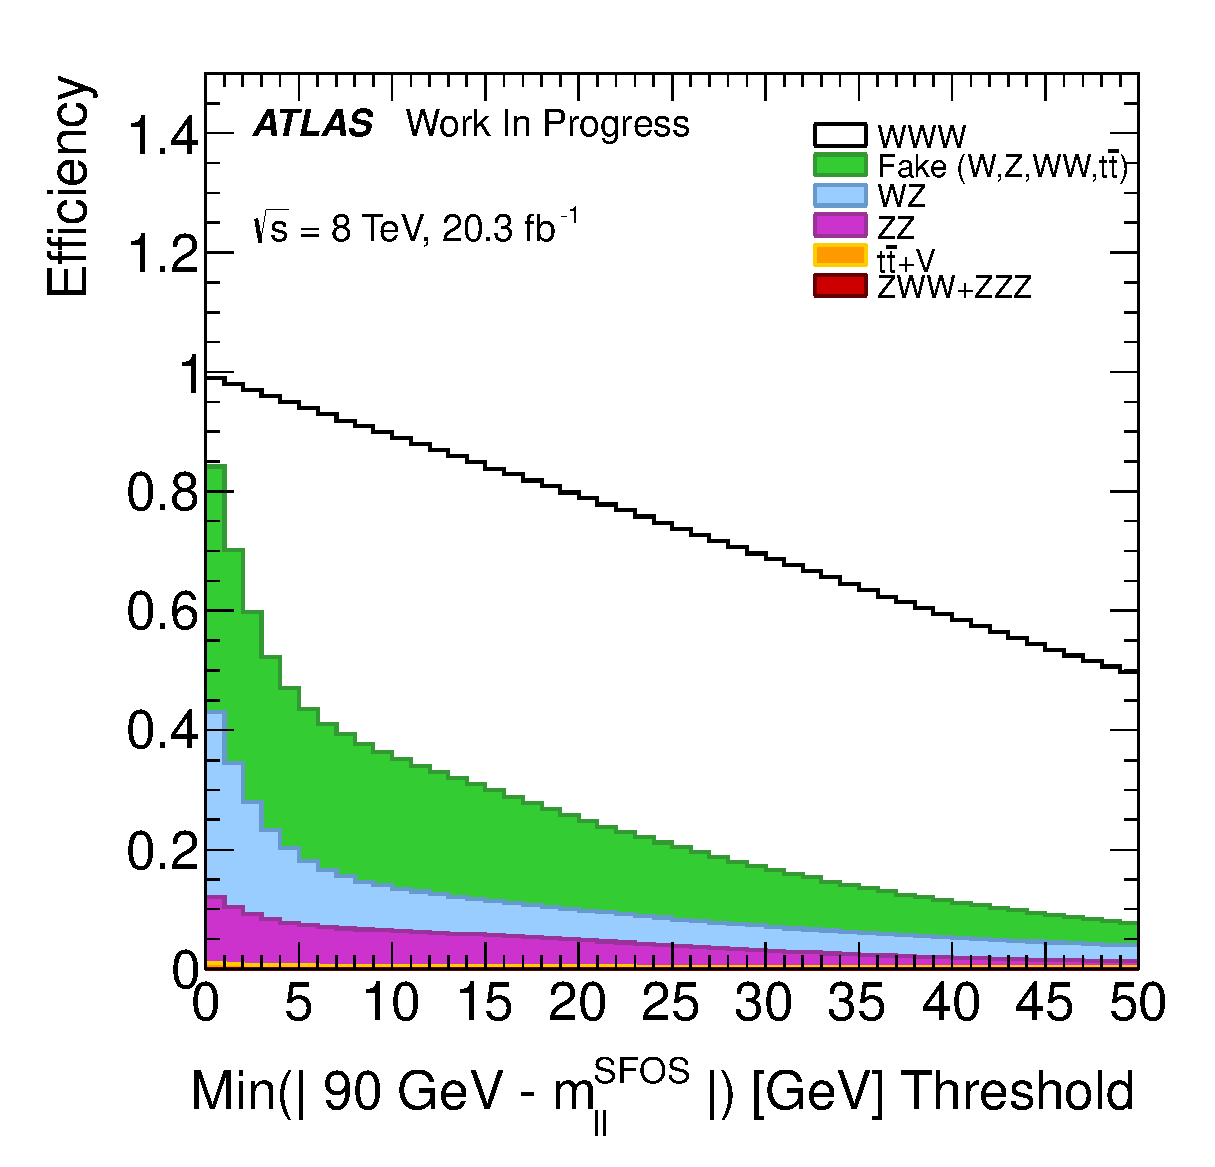
\includegraphics[scale=0.25]{figures/optimization/SignalRegions_0p5mmZ0_Preselection_Efficiencies/ZWindow_Cumulative.eps}
\caption{Signal and background efficiencies as a function of various cuts when starting from event pre-selection.}
\label{fig:optimization_efficiencies_preselection}
\end{figure}



\begin{figure}[ht!]
\centering
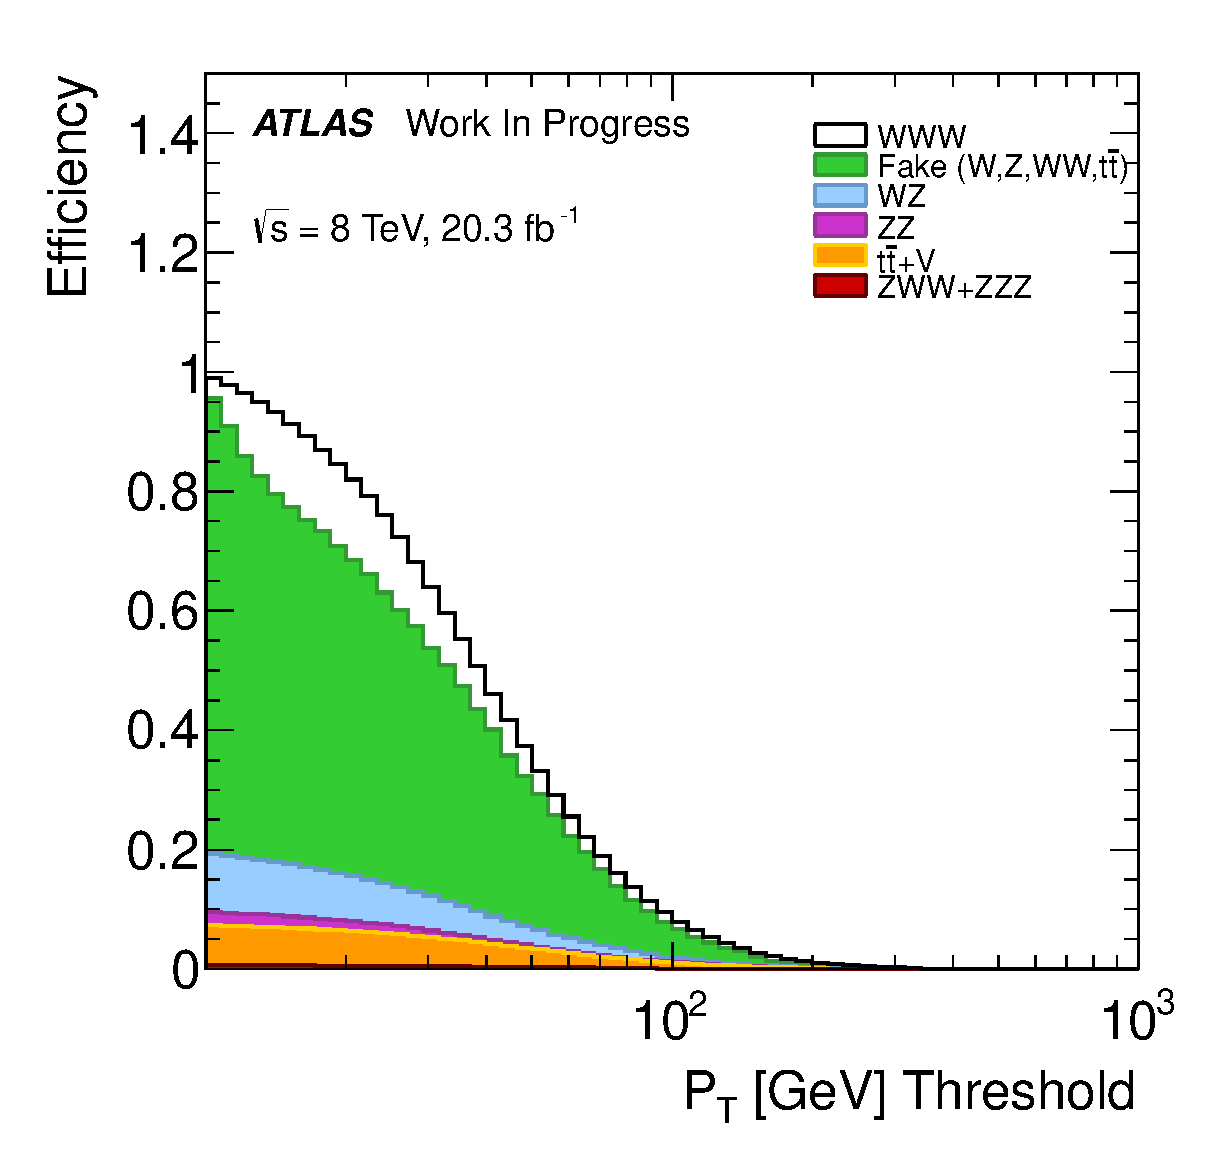
\includegraphics[width=0.3\columnwidth]{figures/optimization/SignalRegionsPreselection_0SFOS_Efficiencies/AllLeptonPt_Cumulative.eps}
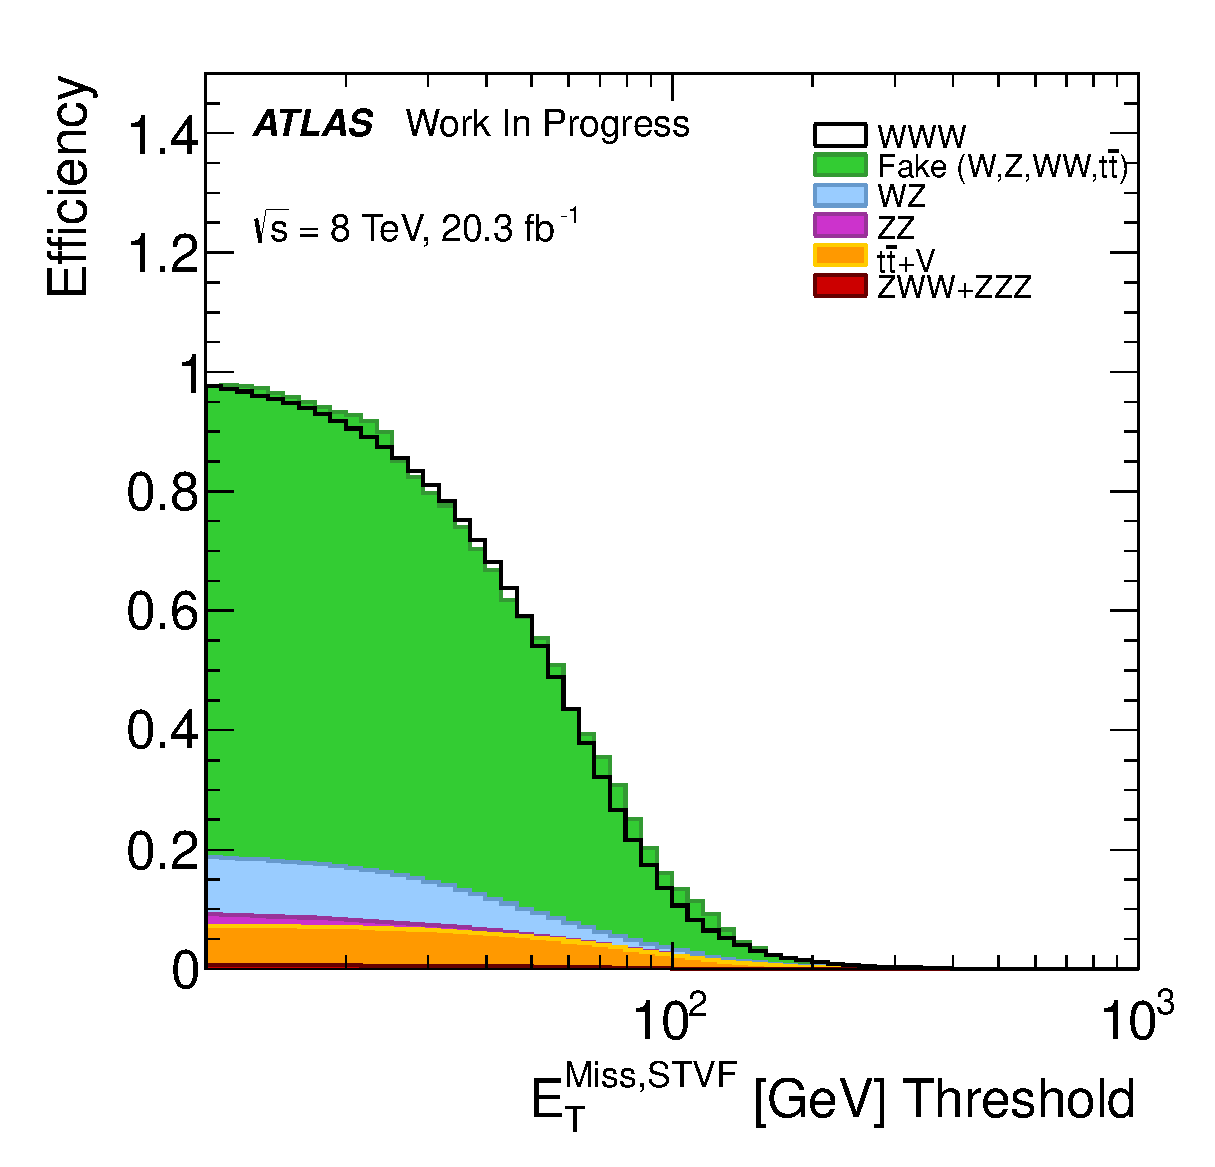
\includegraphics[width=0.3\columnwidth]{figures/optimization/SignalRegionsPreselection_0SFOS_Efficiencies/MET_Et_STVF_Cumulative.eps}
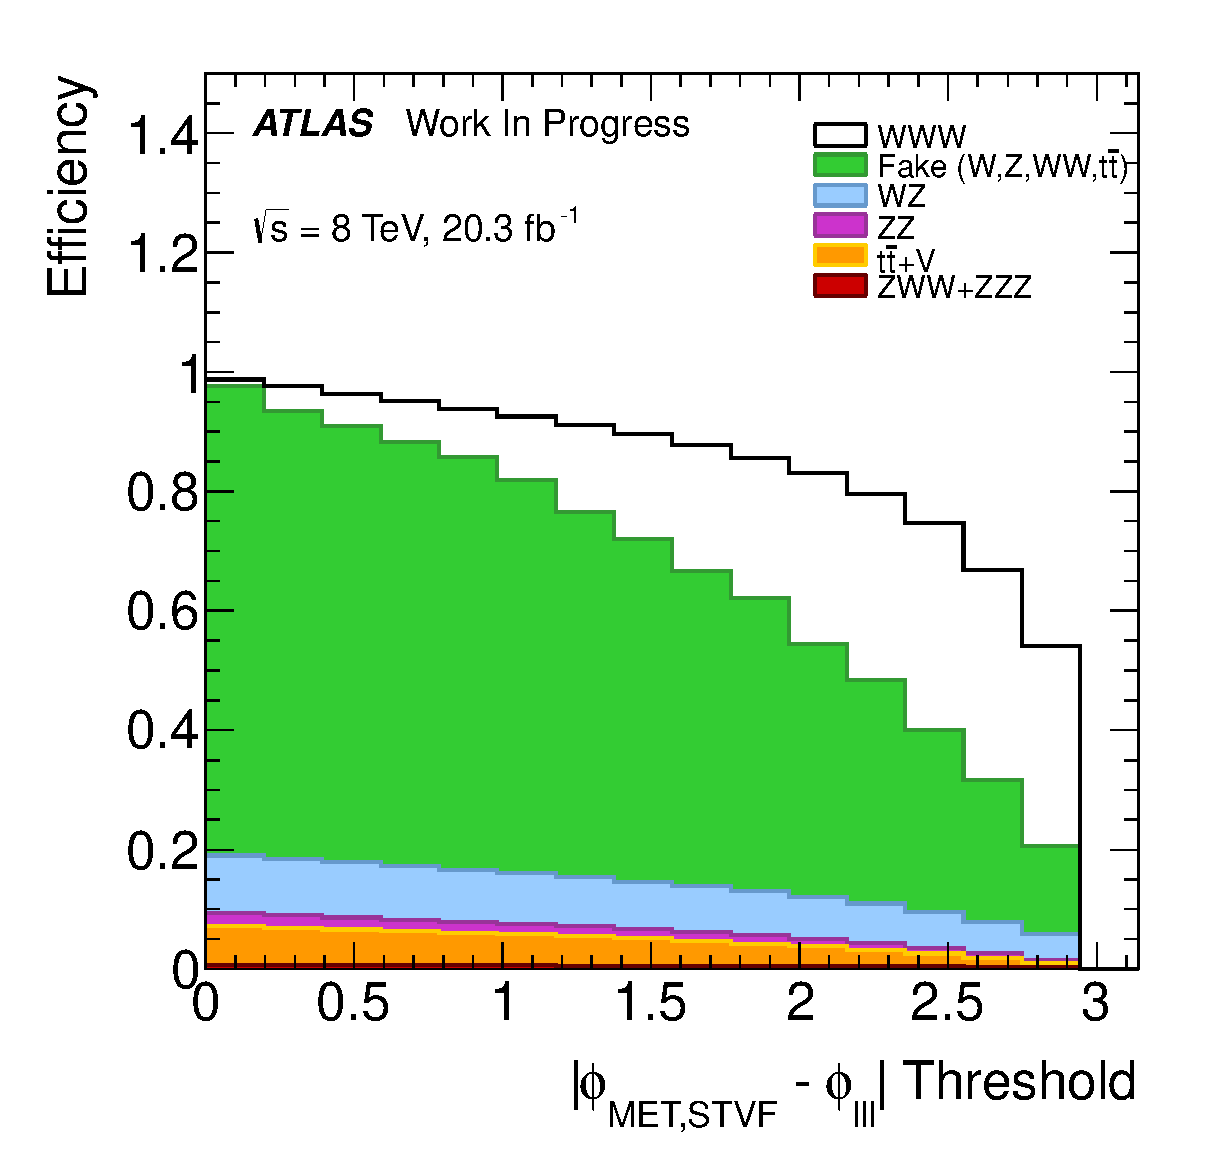
\includegraphics[width=0.3\columnwidth]{figures/optimization/SignalRegionsPreselection_0SFOS_Efficiencies/DeltaPhiMETSTVF123_Abs_Cumulative.eps}
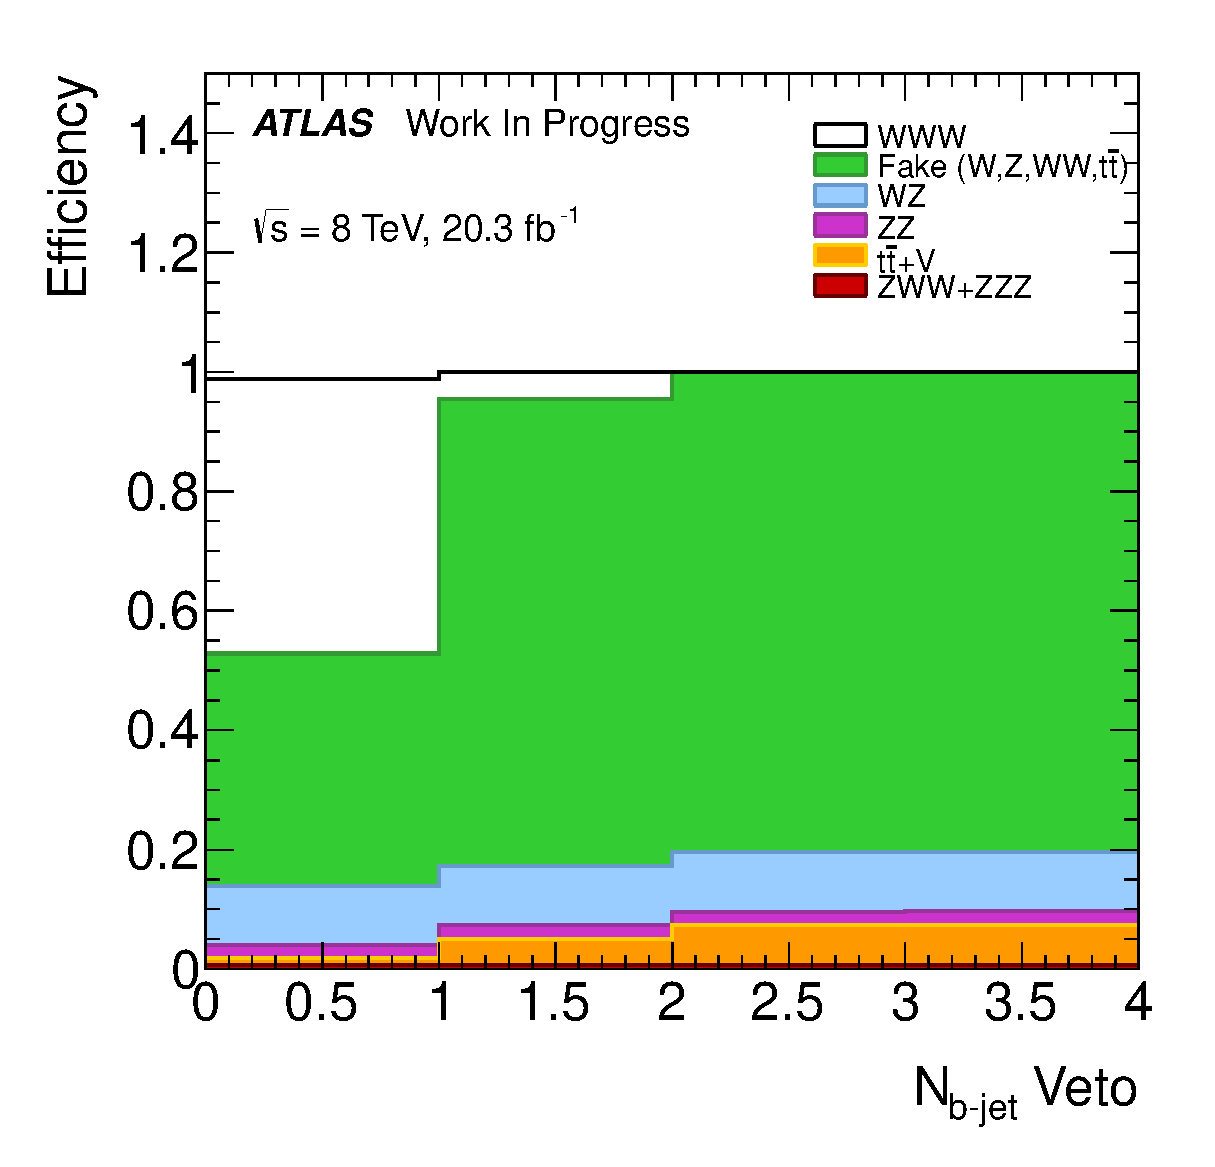
\includegraphics[width=0.3\columnwidth]{figures/optimization/SignalRegionsPreselection_0SFOS_Efficiencies/NBTaggedJets_LeftCumulative.eps}
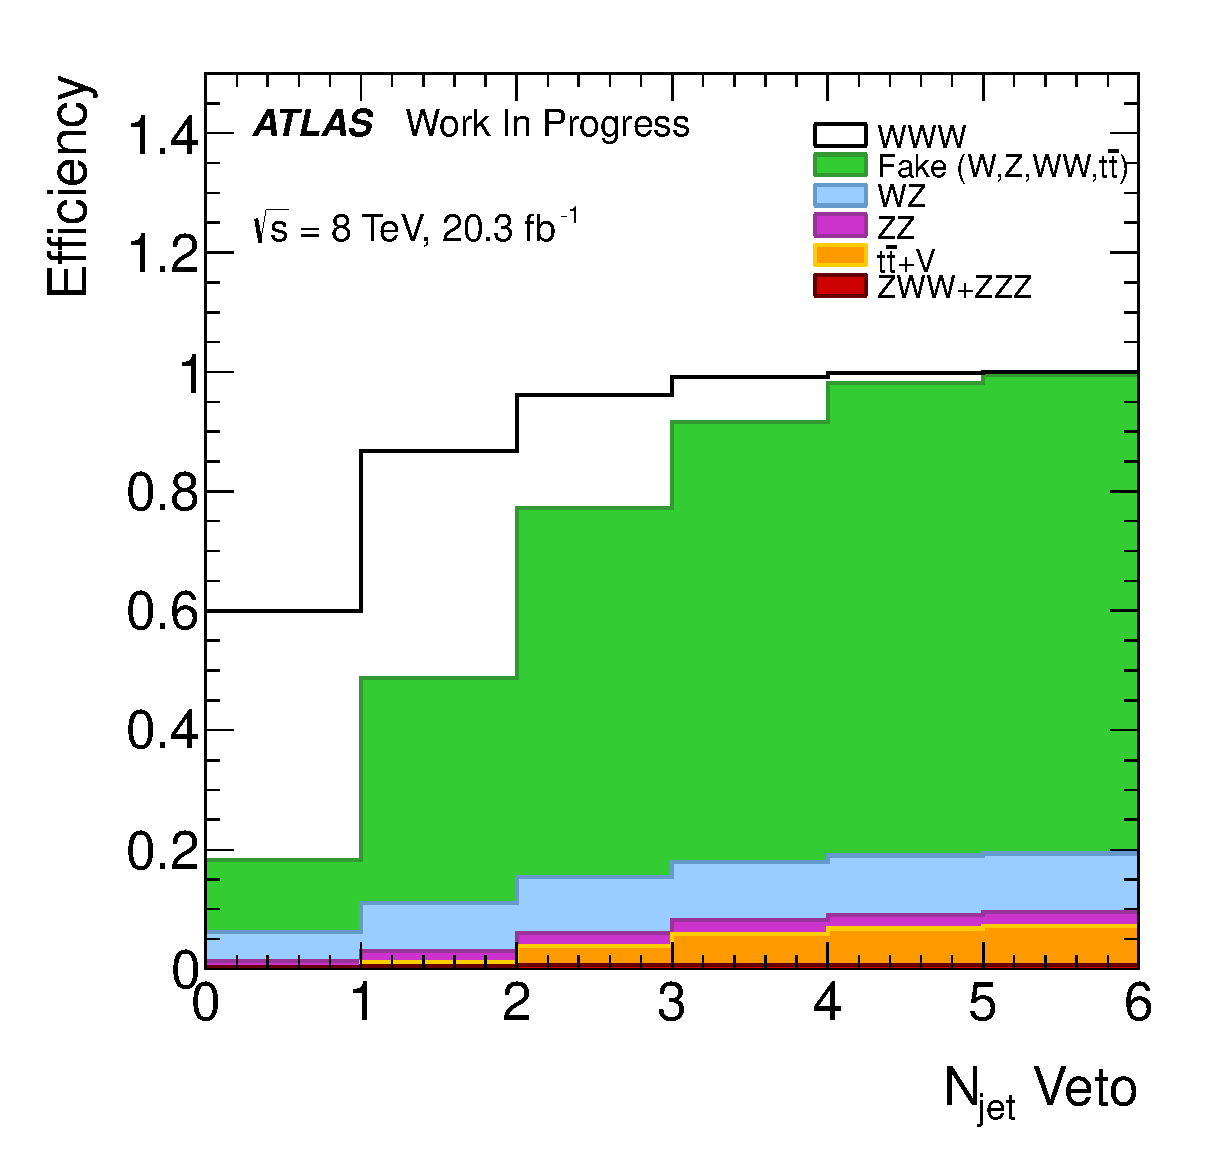
\includegraphics[width=0.3\columnwidth]{figures/optimization/SignalRegionsPreselection_0SFOS_Efficiencies/NJets_LeftCumulative.eps}
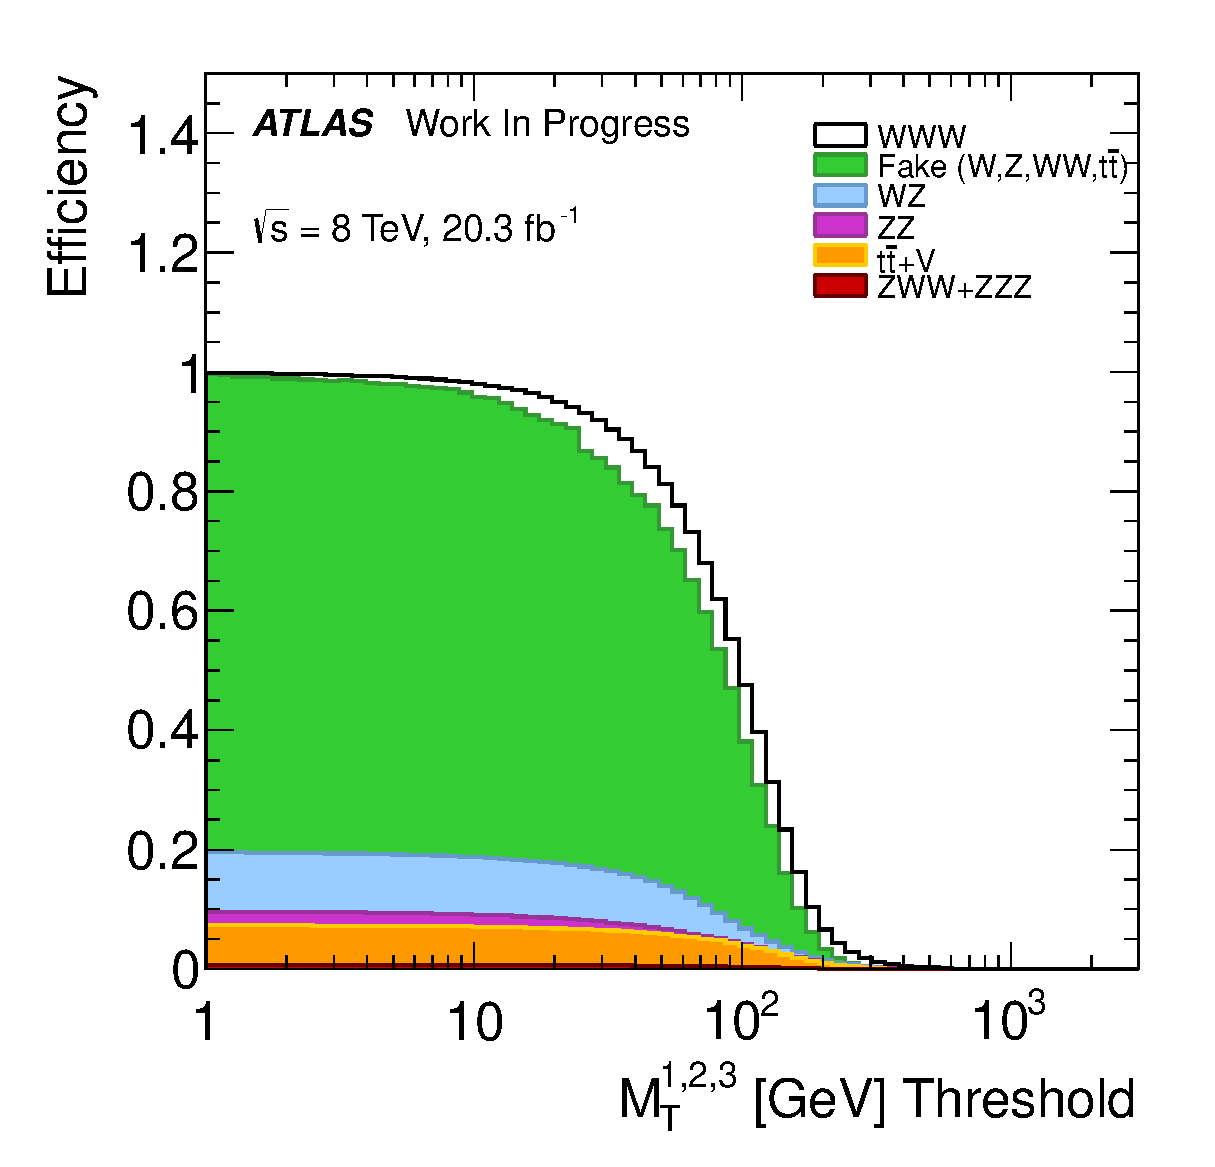
\includegraphics[width=0.3\columnwidth]{figures/optimization/SignalRegionsPreselection_0SFOS_Efficiencies/ThreeLeptonMt_Cumulative.eps}
%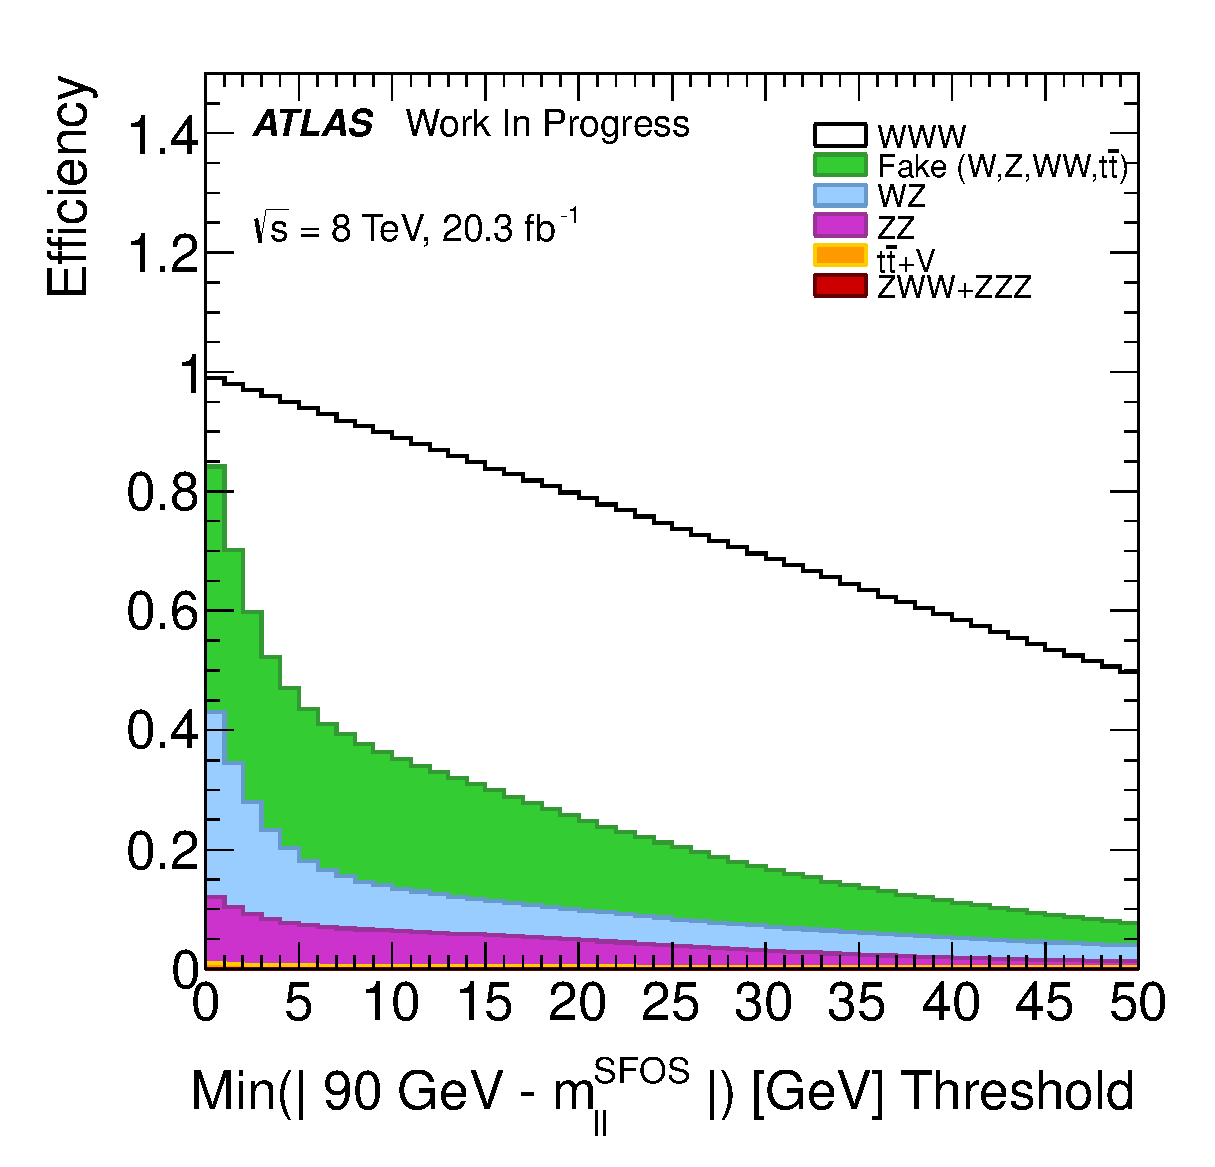
\includegraphics[scale=0.25]{figures/optimization/SignalRegions_0p5mmZ0_Preselection_Efficiencies/ZWindow_Cumulative.eps}
\caption{Signal and background efficiencies as a function of various cuts when starting from event pre-selection + 0 SFOS lepton pairs.}
\label{fig:optimization_efficiencies_0sfos}
\end{figure}

We can plot the efficiency for the signal as well as the background
as a function of the threshold, $X$, for each of these quantities. 
The efficiencies are shown starting 
in the pre-selection region in 
\fig\ref{fig:optimization_efficiencies_preselection} 
(which has a similar background composition to the 1 and 2 SFOS regions)
and in the pre-selection + 0 SFOS region
in \fig\ref{fig:optimization_efficiencies_0sfos}.
Clearly, the shape of the efficiencies between the signal and
background is not always the same, which means that we have some
power to reduce the background with respect to the signal.
Furthermore, these shapes are not the same in the pre-selection 
+ 0 SFOS region as they are in just the pre-selection region.
For instance, in the 0 SFOS region, the shape of the efficiencies
for signal and background are very similar as a function
of the \MET~threshold, but in the pre-selection stage they are
very different, with the background efficiency dropping much
more rapidly than the signal efficiency. This suggests that
a cut on the \MET~distribution could be very useful 
in the 1 and 2 SFOS regions but not in the 0 SFOS region.
Something similar may be true for a cut on $m_{T}^{lll}$.
On the other hand, a cut on \deltaphi~ could prove useful in all 
signal regions. The lepton \pt~is frequently used as a useful discriminant
but in this case it seems to rapidly remove the signal at about the
same rate as the background, so a tighter cut on the lepton \pt~
is likely to prove to be not useful. Cuts on \njet~seem to remove a lot of 
the signal but cut tighter on the background in the pre-selection
+ 0 SFOS region, which could prove useful.  Most impressive is 
the cut on \nbjet, which leaves the signal efficiency at almost exactly
one, while having a large impact on the pre-selection + 0 SFOS region
where the fake contribution is large.

This type of heuristic study  can be used to obtain insight into
the distributions that are useful for discriminating 
between signal and background.  But using these distributions
alone to determine a final selection is a little haphazard.
For one, they do not tell us the impact that cutting on multiple
distributions will have.  These distributions are likely to be 
at least partially correlated, so that cutting on one distribution might
enhance or deflate the impact of another cut. 
And two, it is not at all clear from these distributions
what is the best choice of cuts. We need a metric that will
allow us to make decisions about which cuts to choose.
The metric to use should be one that is 
related to the final prediction after all selection cuts are applied.
Thus, the metric cannot be used to make a decision about each 
cut individually, but instead about some combination of cuts.

To deal with the issues mentioned above, we 
decided on the final signal region selection using an optimization
procedure. The optimization takes as input a multi-dimensional 
space where each dimension is the selection threshold
for one of the quantities listed above, plus some others not mentioned.
The range of the multi-dimensional space that is 
is restricted so that the 
predicted signal remains finite i.e. non-zero.
At an individual point in this space, the optimization computes
the expected signal and background events after the selection
along with the size of statistical uncertainties
and systematic uncertainties on the model. 
These are then used as input to the measurement extraction framework
described in \sec\ref{} to determine the width of the precision
on the final measurement. 
This width is used as the metric to minimize in the optimization.
By considering a metric like this, we are optimizing directly
the quantity of interest to the final measurement, and taking
into account not just the individual predictions, but also their
uncertainties. This is important because it can more stringently
remove backgrounds that have large uncertainties.

We choose to treat the sample space as being discrete as opposed
to continuous. For some dimensions of the space, such as 
the threshold on \njet, this is manifestly true, as there 
can only be an integer number of observed jets. 
For other dimensions, such as the threshold on the lepton
\pt, these quantities are real valued and thus continuous.
However, looking at \fig\ref{fig:optimization_efficiencies_preselection} 
and \fig\ref{fig:optimization_efficiencies_0sfos}, the shape
of the efficiencies tend to change relatively slowly from bin
to bin. Thus, it should be acceptable to only sample 
discretely as long as they can capture the shape information of 
the efficiencies as they do above. Furthermore, 
this acknowledges the finite  experimental resolution of these 
quantities. For example,
the difference between $\pt > 20~\GeV$ and $\pt > 20.5~\GeV$
should not be taken too seriously because of the effects of limited
track and energy resolution used to derive the muon and electron \pt.
%expand on this? what would be the typical electron and muon resolution here?
Treating the sample space as discrete means that the optimization
function is not smooth and so cannot readily take into account
derivative information to be used for instance 
in some sophisticated minimization algorithm.
Fortunately, the number of points in the sample space after discretizing, 
while large, is small enough that it can be evaluated in its entirety
using a brute force approach. Thus, we choose to evaluate the 
optimization in the restricted and discretized sample space in order
to find an optimal choice for the selection.

%I should redo the optimization for the specific bin sizes and list them

The shape of the optimization can be seen in \fig\ref{fig:optimization}.
\emph{Figures need to be reproduced. Elaborate...} 


\begin{figure}[ht!]
\centering

\includegraphics[width=0.3\columnwidth]{figures/placeholder.eps}

\includegraphics[width=0.3\columnwidth]{figures/placeholder.eps}

\includegraphics[width=0.3\columnwidth]{figures/placeholder.eps}
\caption{Signal Yield vs Measurement Uncertainty for optimized points 
in the 0 SFOS (left), 1 SFOS (middle), and 2 SFOS (right) signal regions.}
\label{fig:optimization}
\end{figure}



\begin{table}[ht!]
\centering
\begin{tiny}
\begin{tabular}{|c||c||c||c|}
\hline
&  0 SFOS  	& 1 SFOS		  & 2 SFOS  \\
\hline 
\hline 
\multirow{2}{*}{Pre-selection} & \multicolumn{3}{c|}{Exactly 3 leptons with $P_{T} > 20$~GeV}\\
                               & \multicolumn{3}{c|}{where at least one is trigger matched.  (See Section~\ref{sec:preselection}) }\\
%\hline
%Lepton $P_{T}$ 	&       \multicolumn{3}{c|}{$P_{T} > 20$~GeV}   	  \\
\hline 
b-tagged Jet Veto	& \multicolumn{3}{c|}{$N_{b-jet} = 0$ (85 \% b-tagging efficiency)} \\
\hline 
Same-Flavor Mass &	$m_{\textrm{SF}} > 20$~GeV	& \multicolumn{2}{c|}{} \\
\hline 
Z-Veto                &  $|m_{ee}-m_Z|$ & $m_{\textrm{SFOS}} < m_{Z}-35\GeV$ & $|m_{\textrm{SFOS}}-m_Z|$ \\
($m_Z = 91.1876\GeV$  &  $>15\GeV$                                         & OR   &  $>20\GeV$\\
                      & 					  & $m_{\textrm{SFOS}}>m_{Z}+20\GeV$	   &  \\
%Z-Veto                &  \multirow{3}{*}{$|m_{ee}-m_Z| > 15$~GeV} & $m_{\textrm{SFOS}} < m_{Z}-35\GeV$ & \multirow{3}{*}{$|m_{\textrm{SFOS}}-m_Z| > 20$~GeV} \\
%($m_Z = 91.1876\GeV$  &                                           & OR                                     &  \\
%                      & 					  & $m_{\textrm{SFOS}}>m_{Z}+20\GeV$	   &  \\
\hline 
Missing $E_{T}$		& 		& $E_{T}^{Miss} > 45$~GeV & $E_{T}^{Miss} > 55$~GeV \\
\hline 
Lepton-Missing $E_{T}$ Angle 	& 	\multicolumn{3}{c|}{$|\phi(3l)-\phi(E_{T}^{Miss})| > 2.5$} \\
\hline 
Inclusive Jet veto	& \multicolumn{3}{c|}{$N_{jet} \leq 1$} \\
\hline 
\end{tabular}

\end{tiny}
\caption{Optimized signal selection split by number of Same-Flavor Opposite-Sign (SFOS) lepton pairs.}
\label{tab:signal_selection}
\end{table}

%other metrics like what?


%I would like to show some plots demonstrating the effect of the optimization
%One way is that I could just show all of the different points evaluated
%with their uncertainty and signal like I have shown before. 
%It might be nice to as well overlay some isoforms for different
%constant selections which could give a nice idea of the effect of diff. selections.
%But perhaps there are even better ways to visualize the effect of a 
%multi-dimensional optimization function


%It should be said that a more algorithmic way of choosing the type 
%of quantities to consider could improve this selection. Deep learning...



From the optimization, a final selection is chosen separately for each signal
region.  This selection is presented in \tab\ref{tab:signal_selection}.
In all regions, a veto is applied on events with jets tagged to come from \bee~
or \bee-hadron decays. Besides the nominal \bee-tagging operating
point with an 85~\% \bee-tagging efficiency (mentioned in
\sec\ref{sec:object_selection}), other 
\bee-tagging efficiency operating points
were considered that had a lower efficiency (namely 80\%, 70\%, and 60\%). 
These other operating points could be useful if the \bee-tagging mis-identification
was high enough to remove a significant portion of the signal. However,
even at the 85~\% operating point
the mis-identification efficiency remains manageable at about 1~\%. 
Even with some jet mis-identification, the signal has
a very high efficiency of passing this 
cut of $> 99$~\% while offering some of the strongest 
reduction in the fake lepton background. 
Thus there is no benefit observed by going to a lower efficiency operating point.
The analysis could potentially benefit from an even more stringent 
operating point, but the highest
efficiency operating point that is supported by the ATLAS
\bee-tagging group is the 85~\% efficiency operating point.
In addition to the the \bee-jet veto, there is an additional
cut on the jet multiplicity, regardless of whether or not 
the jet is tagged. By only keeping
events with no more than one jet, 
the signal efficiency is almost $90$~\% while reducing
the background by about 50~\%.  Applying a veto on 
all jets does a very good job at removing the fake lepton
background, but the signal efficiency is prohibitively small, at about 60~\%. 


%should this description be moved earlier
Some of the backgrounds include the production of \z~bosons.
The invariant mass of the \z-boson can be reconstructed from the SFOS
pair coming from the \z-boson decay. This will result in a peak from these backgrounds
in the invariant mass distribution around the $Z$-mass ( $m_{Z}=91.1876$~GeV \cite{PDG:2014}).
The signal, which does not include $Z$-bosons, will not have the same peak, but instead
will be relatively flat around the region of the $Z$-peak. 
This can clearly be seen in the plot of $m_{\textrm{SFOS}}$ in \fig\ref{fig:preselection}.
As a result, removing events within some window around the peak can do a good job
of removing these backgrounds without having a large effect on the signal.
In the 0 SFOS region, by definition there are no SFOS pairs that could come 
from the decay of a \z-boson. However, the effect of electron charge mis-identification,
discussed in \sec\ref{}, means that a peak can show up in the background
of the $m_{ee}$ distribution for same-sign electron/positron pairs. 
This can clearly be seen in \fig\ref{}.
Thus, a veto can be performed in this distribution as well.

The presence of neutrinos in the signal mean that the signal should have a 
relatively large \MET~compared to most of the backgrounds. Thus, 
cutting on the \MET~distribution such that it is large can remove backgrounds
expected to have small \MET, like $Z\gamma$ production.
Still, there are some large backgrounds with neutrinos, like $WZ$, 
and also backgrounds that have contributions to the \MET from objects that have
missed reconstruction, like $ZZ$, which can also have a moderate to large \MET.
Thus, some care must be taken to choose a threshold to cut on the \MET.

\begin{figure}[ht!]
\centering
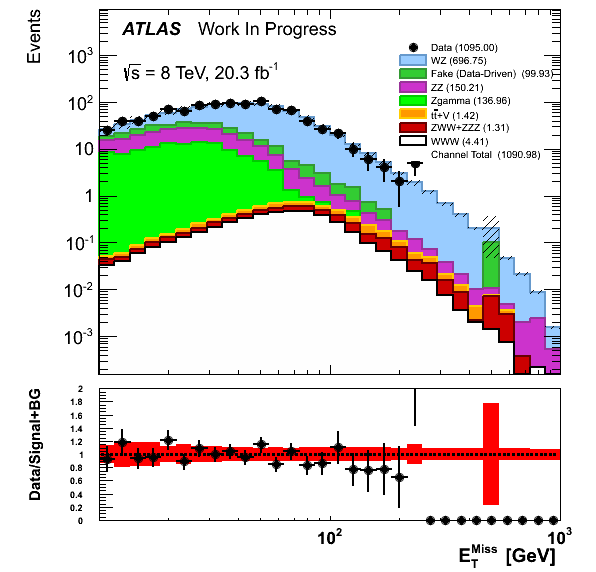
\includegraphics[width=0.4\columnwidth]{figures/appendix_signal_selection/Nov24Update_FakeSys_KFacSys_LogY_NoRebin/output/jobs/MxM/DataFull_Rates_May13_FakeRatesExactly2Loose_MuonMxMBJetGt0_ElBJetGt0SubtractPC_MxM/PreselectionNov23_15_1SFOS_ChargeAbs1_BVeto85_physics/weight_all/png/MET_Et_histratio.png}
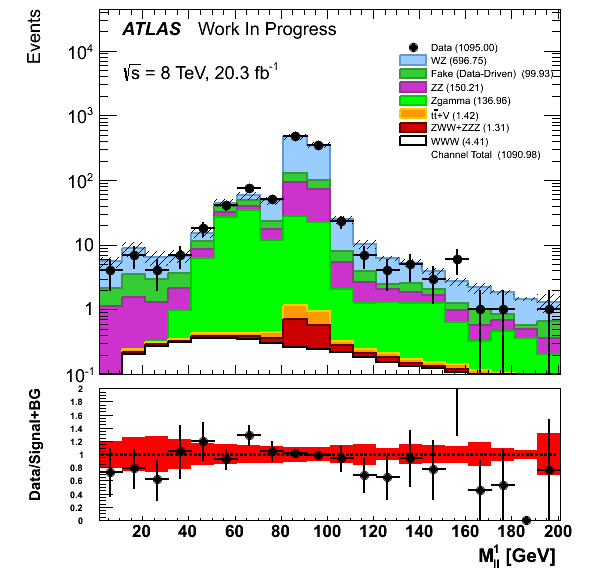
\includegraphics[width=0.4\columnwidth]{figures/appendix_signal_selection/Nov24Update_FakeSys_KFacSys_LogY_NoRebin/output/jobs/MxM/DataFull_Rates_May13_FakeRatesExactly2Loose_MuonMxMBJetGt0_ElBJetGt0SubtractPC_MxM/PreselectionNov23_15_1SFOS_ChargeAbs1_BVeto85_physics/weight_all/png/InvariantMassSFOS_histratio.png}
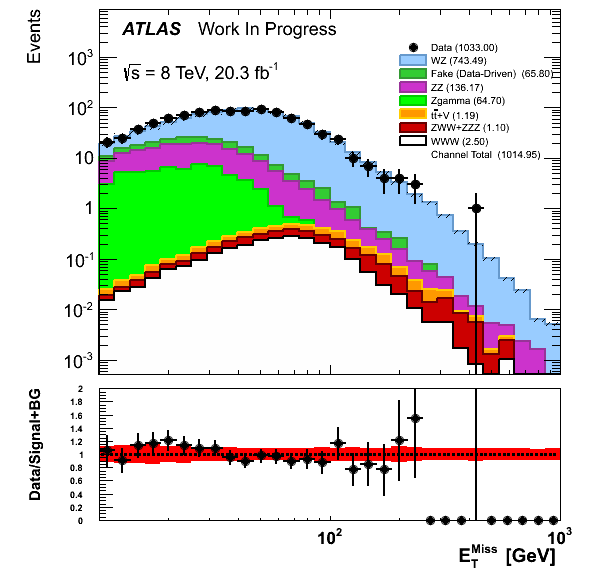
\includegraphics[width=0.4\columnwidth]{figures/appendix_signal_selection/Nov24Update_FakeSys_KFacSys_LogY_NoRebin/output/jobs/MxM/DataFull_Rates_May13_FakeRatesExactly2Loose_MuonMxMBJetGt0_ElBJetGt0SubtractPC_MxM/PreselectionNov23_15_2SFOS_ChargeAbs1_BVeto85_physics/weight_all/png/MET_Et_histratio.png}
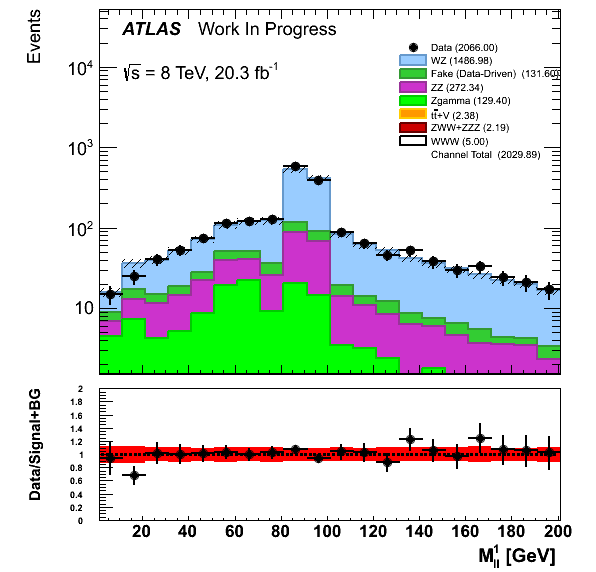
\includegraphics[width=0.4\columnwidth]{figures/appendix_signal_selection/Nov24Update_FakeSys_KFacSys_LogY_NoRebin/output/jobs/MxM/DataFull_Rates_May13_FakeRatesExactly2Loose_MuonMxMBJetGt0_ElBJetGt0SubtractPC_MxM/PreselectionNov23_15_2SFOS_ChargeAbs1_BVeto85_physics/weight_all/png/InvariantMassSFOS_histratio.png}
\caption{Plots of the \MET (left) and $m_{\textrm{SFOS}}$ (right) distributions 
in the 1 SFOS (top) and 2 SFOS (bottom) regions after pre-selection
plus the \bee-veto requirement.}
\label{fig:met_zwindow_optimization}
\end{figure}

The $Z\gamma$ background shows up in the low-shoulder of the \z-peak
in the $m_{\textrm{SFOS}}$ distribution and at low MET. This can be
seen both for the 1 and 2 SFOS regions in \fig\ref{fig:met_zwindow_optimization}.
As a result, the $Z\gamma$ background can be removed either by tuning 
the \z-mass window used in the veto above, or by removing events with low \met.
Thus, the optimization shows that there is some correlation 
between the \z-veto window and the \met~selection threshold. 
In the 1 SFOS region, there is a larger 
contribution from $Z\gamma$ processes than in the 2 SFOS
region.  This process mostly shows up in the low shoulder 
of the \z~ peak. The optimization
prefers removing this $Z\gamma$ contribution by setting an 
asymmetric \z-window in the 1 SFOS
region, with the boundaries being 35~GeV below the \z-pole 
and 20~GeV above and then keeping the \MET cut a little loose, with a 
threshold of $\MET > 45$~GeV.  Meanwhile, in the 2 SFOS region,
the $Z\gamma$ contribution is not as prominent and the 
optimization happens to prefer a symmetric
window of $\pm20$~GeV around the \z-pole.  
The looser \z-veto then allows for a tighter
missing $E_{T}$ cut with a threshold of $\MET > 55$~GeV. 
In the 0 SFOS region there 
are no SFOS pairs by definition,
but there is still a peak in the same-sign electron-electron mass 
distribution due to charge mis-identification.
The optimization prefers a slightly narrower symmetric window 
of $\pm15$~GeV around the \z-mass. 
Further, as already mentioned,
this background turns out 
to have a similar missing $E_{T}$ distribution
as the signal. As a result, cutting on the missing $E_{T}$ in this region 
offers little to no discriminating power
between the signal and background so we have chosen not to apply 
any cut here in order to maximize the signal yield.


%this description probably belongs in an earlier section
The magnitude and direction
of the missing $E_{T}$ may be interpreted as coming from the 
vector sum of the neutrinos.  By arguments of 
symmetry, one could then compare the azimuthal direction 
of the missing $E_{T}$ to the azimuthal direction of the vector
sum of the three charged leptons. When doing so, one finds that 
in the transverse plane, 
the direction of the three charged leptons
tends to be back-to-back with the direction of the 
three neutrinos (missing $E_{T}$). The
backgrounds also show this behavior, but it is less pronounced than 
it is for the signal.  As a result, 
there is some discriminating power when cutting on the difference 
in the two angles: 
$|\Delta\phi(3l,\MET)| = |\phi(3l)-\phi(\MET)|$. 
The behavior of this quantity for signal and
background is similar in all three signal regions so based on the 
optimization it was chosen to apply the cut
$|\Delta\phi(3l,\MET)| > 2.5$ everywhere.  
We also considered taking the difference in angle between
the missing $E_{T}$ and individual leptons (e.g. the highest $\pt$ lepton) 
but this was shown to be not nearly as effective.  

Finally, the distribution of the invariant mass
from same-flavor lepton pairs (regardless of sign) 
was considered in the 0 SFOS 
region to remove any low-mass contamination from processes like from QCD.  
This was shown to offer some
modest discriminating power and a threshold of $m_{SF} > 20$~GeV 
was chosen only for the 0 SFOS region.

\subsection{Fiducial Region Selection}
\label{sec:fiducial}

A fiducial phase space or fiducial region is the 
region the analysis is sensitive to, defined 
using purely truth information (generator information before
being passed through ATLAS reconstruction).
We define our fiducial region
based on the optimized signal selection (defined at the reconstruction level)
but using only truth information. For instance, the reconstructed
lepton \pt~ requirement of 
$\pt^{\textrm{Reco}} > 20~\GeV$
is taken into account in the fiducial region selection
by requiring 
$\pt^{\textrm{Truth}} > 20~\GeV$.
By applying this for all cuts in the reconstruction selection
shown earlier in \tab\ref{tab:signal_selection},
one may compare the predicted signal yields after reconstruction
using this selection to the one in the fiducial region selection
using just truth information. Any differences are then attributed solely
to effects from reconstruction. 
The fiducial selections are determined at truth level 
using Rivet~\cite{Buckley:2010ar}, which allows for 
comparisons between different generators.


\begin{table}[ht!]
\centering
\begin{tiny}
\begin{tabular}{|c||c||c||c|}
\hline
&  0 SFOS  	& 1 SFOS		  & 2 SFOS  \\
\hline 
\hline 
All & \multicolumn{3}{c|}{All} \\
\hline 
Tau Veto & \multicolumn{3}{c|}{$N_{\tau} < 1$} \\
\hline 
Fiducial Leptons & \multicolumn{3}{c|}{Exactly 3 leptons with $p_{T} > 20~\mathrm{GeV}$ and $|\eta|<2.5$} \\
\hline 
Lepton Overlap Removal & \multicolumn{3}{c|}{$\Delta R(\ell \ell) > 0.1$}\\
\hline 
Same-Flavor Mass &	$m_{\textrm{SF}} > 20$~GeV	& \multicolumn{2}{c|}{} \\
\hline 
Z-Veto                &  \multirow{2}{*}{$|m_{ee}-m_Z| > 15$~GeV} & No $m_{\textrm{SFOS}}$ with  & \multirow{2}{*}{$|m_{\textrm{SFOS}}-m_Z| > 20$~GeV} \\
($m_Z = 91.1876$~GeV) & 					  & $m_{Z}-35 \textrm{GeV} < m_{\textrm{SFOS}}<m_{Z}+20$~GeV	&  \\
\hline 
Missing $E_{T}$		& 		& $E_{T}^{Miss} > 45$~GeV & $E_{T}^{Miss} > 55$~GeV \\
\hline 
Lepton-Missing $E_{T}$ Angle 	& 	\multicolumn{3}{c|}{$|\phi(3l)-\phi(E_{T}^{Miss})| > 2.5$} \\
\hline 
Inclusive Jet veto	& \multicolumn{3}{c|}{$N_{jet} \leq 1$ with fiducial jets of $p_{T} > 25~\mathrm{GeV}$ and $|\eta| < 4.5$ } \\
\hline 
\end{tabular}

\end{tiny}
\caption{Fiducial regions based on optimized selection.}
\label{tab:fiducial_selection}
\end{table}

The chosen fiducial region selection 
is listed in \tab\ref{tab:fiducial_selection}.
Only prompt leptons (those not originating from hadron decays) are used for 
lepton selections, and these leptons are dressed with prompt photons 
within a cone with $\Delta R = 0.1$. Generator-level jets are 
reconstructed by running the anti-kt algorithm with radius 
parameter $\Delta R = 0.4$ on all final-state particles 
after the parton showering and hadronization with the exception of prompt 
leptons, prompt photons, and neutrinos. The \MET~variable is calculated 
using all generator-level neutrinos. 
As can be seen, the selection 
in \tab\ref{tab:fiducial_selection} looks very similar to that in 
\tab\ref{tab:signal_selection} except for the object definitions
using truth information and that 
events are removed if $\tau$ leptons are present from the $W$ decays.  
Thus, the fiducial selection
does not include the branching fraction to $W\rightarrow\tau\nu$ decay, 
even though there will be some contamination from this process in the final 
reconstruction level selection. 



The fiducial cross-sections are evaluated in both 
the \vbfnlo~and \madgraph~samples mentioned in Section~\ref{sec:signal}.
The predicted fiducial cross-sections at each stage of the selection
are listed for both generators in \tab\ref{}.
The fiducial cross-sections and their
statistical uncertainties 
are summarized in each channel for both generators 
after the entire fiducial selection
in \tab\ref{tab:fiducial_cross_sections}.
They are seen to be in good agreement between both generators.


The derived fiducial cross-sections using the two generators are 
shown in Table~\ref{tab:fiducial_cross_sections}.  The cross-sections are observed
to be in good agreement between the two generators. The MadGraph NLO
fiducial cross-sections are used in the final measurement.
The PDF and scale uncertainties on the fiducial cross-sections
are determined after summing over all three signal regions 
as described earlier in \sec\ref{sec:signal}.
% it would probably be a good idea to include the fiducial cut-flows as well.





\begin{table}[ht!]
\centering
\begin{footnotesize}
\begin{tabular}{|c||c|c|}
\hline
        & \multicolumn{2}{|c|}{Fiducial Cross-section [ab]} \\
Channel & MadGraph & VBFNLO \\
\hline\hline
0 SFOS &  $114.7 \pm 4.3$     & $126.9 \pm 1.0$      \\
1 SFOS &  $126.6 \pm 4.3$     & $126.1 \pm 1.0$       \\
2 SFOS &  $50.2 \pm 2.7$     & $50.62 \pm .66$       \\
\hline
\end{tabular}

\end{footnotesize}
\caption{Fiducial cross-sections derived in each signal region for the two generators. Production modes are summed together to get one fiducial cross-section per channel per generator. The cross-sections are seen to be in good agreement
between the two generators.}
\label{tab:fiducial_cross_sections}
\end{table}
